\documentclass[10pt,twocolumn]{article}
\usepackage[top=0.75in,bottom=0.75in,left=0.68in,right=0.68in,columnsep=0.22in]{geometry}
\usepackage{mathtools}
\usepackage{times}
\usepackage{amsmath,amssymb,amsthm}
\newtheorem{proposition}{Proposition}
\theoremstyle{plain}
\usepackage{graphicx}
\usepackage{booktabs}
\usepackage{array}
\usepackage{caption}
\usepackage[colorlinks=true,citecolor=blue!55!black,urlcolor=blue!55!black,linkcolor=blue!55!black]{hyperref}
\usepackage{titlesec}
\usepackage{enumitem}
\usepackage{balance}
\usepackage{listings}
\usepackage{xcolor}

\titlespacing*{\section}{0pt}{5pt}{2pt}
\titlespacing*{\subsection}{0pt}{3pt}{1pt}
\setlength{\abovedisplayskip}{3pt}
\setlength{\belowdisplayskip}{3pt}
\setlength{\textfloatsep}{6pt}
\setlength{\intextsep}{5pt}
\titleformat{\section}{\normalfont\large\bfseries}{\thesection}{0.6em}{}
\titleformat{\subsection}{\normalfont\bfseries}{\thesubsection}{0.6em}{}

\lstset{
  basicstyle=\ttfamily\scriptsize,
  backgroundcolor=\color{gray!8},
  frame=single,
  breaklines=true,
  columns=fullflexible,
  keywordstyle=\color{blue!60!black}\bfseries,
  commentstyle=\color{green!40!black}
}

\captionsetup{font=small,labelfont=bf}

\newcommand{\paperTitle}{A Blockchain-Enabled Zero Trust Architecture for Industrial IoT Identity Management: Tiered Continuous Authorization and Quorum-Governed Revocation}

\title{\paperTitle}
\author{
\normalsize Author Name$^{1}$, Author Name$^{2}$ \\
\small $^{1}$Department of Computer Science, University Name, City, Country \\
\small $^{2}$Department of Computer Science, University Name, City, Country \\
\small \texttt{[email protected]}, \texttt{[email protected]}
}
\date{}

\begin{document}
\maketitle

\begin{abstract}
\noindent
Industrial plants combine long-lived devices, brownfield equipment that cannot hold cryptographic keys, several organizations with a stake in every asset, and requests whose consequences range from reading a temperature to rewriting a controller's program. Identity systems built on one certificate authority, session tokens or periodically refreshed revocation lists fit this setting poorly: a revoked device keeps working until a token expires or a list is refreshed, no single party is trusted by all to revoke it, and one trust threshold serves every request. This paper presents a blockchain-enabled Zero Trust architecture for Industrial IoT identity management. Three smart contracts on a permissioned proof-of-authority ledger hold device identities and status, a tiered access policy with an anomaly hard gate and a strict mode for safety-relevant writes, and a quorum-voting revocation governance. Zone gateways decide routine requests locally against replicated ledger state and anchor Merkle roots of their decision logs, while high-consequence requests are decided on-chain; batch revocation supports firmware recalls. We prove immediate revocation on the on-chain path, a bounded exposure on the fast path, replay resistance, attestation unforgeability, key-reuse prevention and governance safety, and characterize when a spoofing attacker is accepted. On an Ethereum Virtual Machine, registration costs about 215k gas, an on-chain decision about 70k, anchoring 54 gas per decision, and a quorum revocation 313k--800k gas for 5--21 voters; batching cuts recall gas by about 40\%. On a synthetic fleet the on-chain path accepted no request after revocation, against 33--147 for token and list baselines. With the behavioural signal taken from real TON\_IoT traffic, the full policy accepted under 1\% of attack requests of seen types at the critical tiers but 6.6--11.9\% of held-out types on average, and 29--77\% when an adaptive attacker sent only its best-scoring flows; telemetry alone was a weak signal. A second dataset from a SCADA testbed showed the same gate behaviour with a supervised detector but a much higher false-denial cost (12--18\% of legitimate requests at the critical tiers) with an unsupervised one. On a four-validator QBFT network (Hyperledger Besu, 2\,s blocks, one host) audited calls were final in about one block period (2.0\,s), a revocation was visible on a second validator in 1.9\,s and denied all 30 later audited requests, a three-of-five quorum revocation took 4--8\,s, and sustained throughput was only 11--18 decisions per second, far below the gas-based ceiling; with two of four validators down the chain halted safely and resumed after recovery. Testbed timings are compute-bound, the network was a single host without wide-area delay, and posture and network signals remain synthetic. Code is released at \href{https://github.com/irfanrazanaqvi/BCZT_IDM_IoT_experments_code}{github.com/irfanrazanaqvi/BCZT\_IDM\_IoT\_experments\_code}.

\noindent\textbf{Index Terms}\textemdash Industrial IoT, Zero Trust Architecture, Blockchain, Decentralized Identifiers, Identity Management, Smart Contracts, Revocation Governance, Operational Technology.
\end{abstract}

\section{Introduction}\label{sec:intro}

\subsection{Motivation}
An industrial plant is a poor fit for the assumptions behind most identity systems. Its devices live for fifteen or twenty years, speak protocols that predate public-key cryptography, sit behind process-critical networks that cannot be rebooted at will, and are administered by several organizations at once: the operator who runs the line, the original manufacturer who ships firmware, an integrator who commissioned the cell, and sometimes an outside maintenance contractor. Guidance for operational technology (OT) security is explicit that availability and safety, not confidentiality, usually dominate the design space, and that a control that interrupts a process can be worse than the attack it prevents \cite{stouffer2023sp80082}. At the same time the attack surface has widened, because IT--OT convergence connects field assets to analytics, remote support and cloud services. Zero Trust, which drops trust based on network location and demands that every access be authenticated, authorized and re-evaluated \cite{nist800207,fernandez2024critical,phiayura2023comprehensive}, is a natural response, and early proposals adapt it to critical OT systems \cite{song2025ztot,zanasi2024flexible}.

Identity is where the difficulty concentrates. A conventional public-key infrastructure gives each device a certificate and relies on revocation lists or short certificate lifetimes to withdraw it. In a multi-party plant, however, there is rarely one party that every other party is willing to let revoke a controller, and the delay between the decision to withdraw a device and the moment every gateway honours it is exactly the window in which a compromised or recalled device keeps working. Blockchain-based identity management addresses the first problem by anchoring identifiers, keys and status on a tamper-evident ledger that several organizations operate together, following the decentralized-identifier (DID) model \cite{w3cdid2022,hosseini2023blockchain,aguru2025ssi,folino2025puf}. Recent industrial work builds authentication on this foundation \cite{zhai2025chebyshev}, and surveys of blockchain for Industrial IoT (IIoT) catalogue its promise and its open problems \cite{essaid2025iiotbc}. Studies that combine blockchain with Zero Trust have followed \cite{liu2024dissecting,nie2025zeroTrust,salim2026ztblociot,mukta2026ztdelegation,jamwal2026survey,farhan2026ztfsf,potturi2026hybrid}.

\subsection{Problem Statement and Gap}
Reading this literature with an operator's eye, three things are missing. First, most blockchain-IoT identity schemes still authenticate once and then treat the session as trusted, which is precisely what Zero Trust is meant to remove \cite{wang2026medicaliot,james2024authz}; and the Zero Trust proposals for industrial settings generally assume one organization owns the policy decision point \cite{kumar2024industry40,zanasi2024flexible}. Second, a single trust threshold is applied to every request, although reading a temperature and rewriting a safety-controller setpoint carry very different consequences; and, as we show analytically and experimentally, a fixed threshold on a weighted score can be unreachable by an attacker who spoofs most of the signals. Third, nearly all of these designs implicitly place every decision on the ledger, which cannot meet the rates and latency of plant networks, and none of them says how a manufacturer's firmware recall, a legacy device that cannot hold a key, or a lost connection to the ledger should be handled. We therefore ask:

\emph{How can a consortium-operated blockchain identity registry be combined with continuous, consequence-aware authorization so that (i) revocation, including large-scale firmware recalls, takes effect without a token or list-refresh window and without any single party being able to impose it, (ii) the strength of verification scales with the criticality of the resource, and (iii) the enforcement path stays fast, available and auditable on industrial networks?}

\subsection{Contributions}
This paper makes the following contributions.
\begin{itemize}[leftmargin=1.1em,itemsep=0pt,topsep=1pt]
  \item \textbf{Architecture.} A zone-aware design (Section~\ref{sec:arch}) with three smart contracts (identity registry, Zero Trust access policy, quorum revocation governance), a tiered policy model that ties the required trust to the criticality of the target resource, an anomaly hard gate and a strict mode for safety-relevant writes, a protocol-gateway identity proxy for legacy devices, and batch revocation and quarantine for firmware recalls.
  \item \textbf{Hybrid enforcement.} A two-path decision model: a fast path in which a zone gateway decides locally against replicated ledger state and anchors a Merkle root of its decision log, and an audited path in which high-consequence requests are decided by the contract itself (Section~\ref{sec:hybrid}).
  \item \textbf{Analysis.} A threat model for plant environments and six proved properties, including a bound on how long a revoked device can still be accepted on the fast path and a result that exactly characterizes what the anomaly gate does and does not stop (Sections~\ref{sec:model}--\ref{sec:security}).
  \item \textbf{Open implementation and measurement.} Solidity 0.8.24 contracts executed on an EVM with measured gas for every operation, including recall and anchoring, plus a Python testbed using real Ed25519 signatures. Experiments report confidence intervals, a revocation-exposure comparison against token and CRL baselines, per-tier attack and false-denial rates, a gate sensitivity study, quorum-governance behaviour for 5--21 voters and recall capacity (Section~\ref{sec:eval}). A further evaluation replaces the synthetic behavioural signal with detector scores on real TON\_IoT traffic, including attack types withheld from training and an adaptive attacker (Section~\ref{sec:real_eval}), repeated on a SCADA dataset (Section~\ref{sec:wustl_eval}) and on an industrial dataset with labelled attack types (Section~\ref{sec:wustl21_eval}). The contracts are also deployed on a four-validator Hyperledger Besu QBFT network, first on one host and then with one validator in each of four Google Cloud regions, where we measure finality, revocation visibility, throughput, quorum voting, batch recall and validator failure (Section~\ref{sec:besu_eval}). We state plainly which results are compute-bound and which remain synthetic.
\end{itemize}

\section{Related Work}\label{sec:related}

\subsection{Zero Trust for Industrial and OT Systems}
Zero Trust architecture is by now well surveyed for IoT. Azad et al.\ cover continuous verification and micro-segmentation \cite{azad2024verify}, James et al.\ review authentication and authorization schemes specifically under a Zero Trust model \cite{james2024authz}, and Nahar et al.\ examine the 6G setting, where device density sharpens per-request overhead concerns \cite{nahar2024survey}. Fern\'andez and Brazhuk caution that ``Zero Trust'' is sometimes a label without a falsifiable architecture behind it \cite{fernandez2024critical}, and Phiayura and Teerakanok supply a migration framework with a maturity model \cite{phiayura2023comprehensive}. For OT in particular, Song et al.\ propose a Zero Trust architecture for critical operational technology systems \cite{song2025ztot}, Zanasi et al.\ a flexible architecture for IIoT \cite{zanasi2024flexible}, and Kumar and Sharma integrate blockchain with dynamic access control for Industry~4.0 without a DID-anchored registry \cite{kumar2024industry40}. These works establish the principles; they leave open who owns revocation in a multi-party plant and how a decision should be audited afterwards.

\subsection{Blockchain Identity and Authentication for IIoT}
Surveys of blockchain-based decentralized identification note limits around revocation latency and interoperability \cite{hosseini2023blockchain}, and a broad review of blockchain in IIoT discusses security and privacy opportunities alongside scalability and integration costs \cite{essaid2025iiotbc}. Aguru and Erukala propose a blockchain self-sovereign-identity framework for standardized IoT identification \cite{aguru2025ssi}, Folino et al.\ tie identity to a physically unclonable function as a hardware root of trust \cite{folino2025puf}, and Ren et al.\ combine self-sovereign identity with Zero Trust for AIoT using selective-disclosure credentials \cite{ren2025aiot}. On the industrial authentication side, Zhai et al.\ design a lightweight scheme for IIoT that combines blockchain with Chebyshev chaotic maps to suit constrained devices \cite{zhai2025chebyshev}. DAXiot shows that DID challenge--response for MQTT can run without a blockchain at about 21\% connection overhead over mutual TLS, but then has no shared revocation ledger \cite{philipp2023daxiot}. For revocation itself, Mazzocca et al.\ propose EVOKE, a cryptographic-accumulator mechanism with about 1.5\,KB of per-device state that spreads revocation epidemically among devices \cite{mazzocca2024evoke}; it complements an on-chain status check rather than replacing it. Kumar et al.\ run a privacy-preserving identity system on a private Ethereum proof-of-authority (PoA) chain in which a decentralized voter group governs identity updates and revocations, and report roughly 3--4\,s for registration and under 5\,s for revocation on the live network \cite{kumar2026privacy}; it is the closest published precedent for our governance contract and the only live-chain figure we compare against.

\subsection{Blockchain--Zero Trust Combinations}
Nie et al.\ pair smart-contract policy enforcement with inner-product encryption for fine-grained access in 6G IoT \cite{nie2025zeroTrust}. Salim et al.\ propose ZT-BlocIoT with dynamic trusted gateways and reinforcement-learning-driven sharding, reporting 2{,}500 transactions per second on 700 nodes at 42\,ms latency \cite{salim2026ztblociot}. Wang et al.\ observe that even Zero Trust--inspired schemes for medical IoT typically authenticate once and then trust the session, and propose blockchain-backed continuous authentication \cite{wang2026medicaliot}; the same gap is what motivates our per-request design in industry. Mukta et al.\ delegate Zero Trust access control through a blockchain, which is close to our policy layer but concerns delegation rather than the device identity lifecycle \cite{mukta2026ztdelegation}. For smart factories, Farhan et al.\ describe a conceptual Zero Trust framework on a consortium chain \cite{farhan2026ztfsf}, and Potturi et al.\ combine AI risk scoring with blockchain-anchored federated identity across cloud, edge and IoT \cite{potturi2026hybrid}. Jamwal et al.\ conclude that blockchain-enabled Zero Trust is still mostly proposed at survey level rather than delivered as benchmarked open code \cite{jamwal2026survey}, and a bibliometric analysis finds blockchain with Zero Trust identity management to be one of the field's most active clusters \cite{liu2024dissecting}. Usama et al.\ add decentralized identity, zero-knowledge proofs and Byzantine-resilient federated learning against AI-driven identity attacks \cite{usama2026multilayer}. Federated learning is also studied as a way to share threat intelligence across industrial sites without exposing raw data \cite{tom2025flcti}; we do not use it, but it is a plausible source for the anomaly signal in Section~\ref{sec:signals}.

\subsection{Off-Chain Dependencies, Cost and Oracles}
Because on-chain controls rest on off-chain facts, the reliability of the data that reaches a contract matters. Shujaa et al.\ stress that device attestation, secure boot and key custody remain off-chain dependencies of any blockchain-IoT security design \cite{shujaa2025enhancing}, and Hassan et al.\ survey the oracle problem, that is, how to bring trustworthy external data to a contract \cite{hassan2023oracle}; our trust oracle is an instance of it, and Section~\ref{sec:disc} discusses its single-key weakness. Smart-contract defects are another risk, reviewed by Wei et al.\ \cite{wei2024quality}. On cost, gas has been studied for Ethereum smart contracts \cite{ta2024gascost} and for IoT access control \cite{hasan2023smartcontract}, DPoS and PBFT-based consensus choices have been proposed for IoT and clinical settings \cite{haque2024scalable,peepliwal2024ztab}, and gasless relaying can spare constrained devices from paying fees \cite{madhwal2025gasless}. Ren et al.\ show for vehicular networks that published trust values can themselves link pseudonyms and propose differential privacy to prevent it \cite{ren2026ditdp}, which matters for any design that exposes scores on a shared ledger.

\subsection{Positioning}
Table~\ref{tab:relatedwork} compares the most relevant systems on five properties that matter in a plant: on-chain revocation, continuous per-request authorization, consequence-aware (tiered) policy, handling of legacy and recall scenarios, and a released artifact. The assessments rest on the abstracts and the parts of the full texts we could read; ``not stated'' means we found no statement, not that the property is absent. To our knowledge none of the reviewed systems reports all five.

\begin{table*}[t]
\centering
\caption{Comparison of representative blockchain and Zero Trust systems for (I)IoT identity}
\label{tab:relatedwork}
\scriptsize
\begin{tabular}{p{3.2cm}p{3.6cm}p{1.6cm}p{1.6cm}p{1.6cm}p{2.1cm}p{1.6cm}}
\toprule
\textbf{System} & \textbf{Core mechanism} & \textbf{On-chain revocation} & \textbf{Per-request authZ} & \textbf{Tiered policy} & \textbf{Legacy / recall} & \textbf{Open artifact} \\
\midrule
Zhai et al.\ 2025 \cite{zhai2025chebyshev} & Blockchain + Chebyshev-map authentication (IIoT) & Not stated & Not stated & Not stated & Lightweight devices & Not stated \\
Song et al.\ 2025 \cite{song2025ztot} & ZTA for critical OT & Not stated & Not stated & Not stated & Not stated & Not stated \\
Zanasi et al.\ 2024 \cite{zanasi2024flexible} & Flexible IIoT ZTA & No & Yes & Partial & Not stated & Not stated \\
Kumar \& Sharma 2024 \cite{kumar2024industry40} & Blockchain + dynamic access control (Industry 4.0) & Not stated & Yes & Not stated & Not stated & Not stated \\
Farhan et al.\ 2026 \cite{farhan2026ztfsf} & ZT on consortium chain (smart factory) & Conceptual & Conceptual & Not stated & Not stated & Not stated \\
Potturi et al.\ 2026 \cite{potturi2026hybrid} & AI risk score + chain-anchored identity & Yes & Yes & Not stated & Not stated & Not stated \\
Salim et al.\ 2026 \cite{salim2026ztblociot} & ZT-BlocIoT (trust + DRL sharding) & Yes & Yes & Not stated & Not stated & Not stated \\
Nie et al.\ 2025 \cite{nie2025zeroTrust} & ZT + inner-product encryption (6G) & Yes & Yes & Fine-grained attributes & Not stated & Not stated \\
Wang et al.\ 2026 \cite{wang2026medicaliot} & Blockchain continuous auth.\ (medical IoT) & Yes & Yes & No & Not stated & Not stated \\
Kumar et al.\ 2026 \cite{kumar2026privacy} & Private PoA identity + voter group & Yes (voter group) & Not stated & No & Not stated & Not stated \\
\textbf{This work} & \textbf{DID registry, tiered ZT contracts, quorum governance, hybrid enforcement} & \textbf{Yes (quorum-governed, batch)} & \textbf{Yes (every call)} & \textbf{Yes (4 tiers, gate, strict)} & \textbf{Proxy identity; batch recall; outage mode} & \textbf{Yes (Solidity + Python)} \\
\bottomrule
\end{tabular}
\end{table*}

\section{Industrial Requirements, System and Threat Model}\label{sec:model}

\subsection{Requirements Specific to Industrial Settings}\label{sec:reqs}
Translating the generic Zero Trust and blockchain-identity goals into a plant yields six requirements that drive the design; they are our reading of OT security guidance \cite{stouffer2023sp80082} and of the identity literature surveyed above, not a standard.
\begin{itemize}[leftmargin=1.1em,itemsep=0pt,topsep=1pt]
  \item \textbf{R1 Multi-party authority.} No single organization (operator, manufacturer, integrator) should be able to unilaterally revoke or reinstate a device.
  \item \textbf{R2 Consequence-aware verification.} The evidence required before a request is accepted must grow with the consequence of the target resource: reading telemetry is not rewriting a controller's program.
  \item \textbf{R3 Predictable, available enforcement.} The common-case decision must be fast and must not depend on the ledger being reachable; consensus latency is acceptable only for rare, high-consequence actions.
  \item \textbf{R4 Brownfield coexistence.} Devices that cannot hold a key or run a signature scheme must be representable without weakening the identities of those that can.
  \item \textbf{R5 Recall at fleet scale.} Withdrawing a vulnerable firmware generation must be possible for thousands of devices in a bounded number of blocks.
  \item \textbf{R6 Auditability.} Every decision, including those taken locally for speed, must be attributable and tamper-evident after the fact.
\end{itemize}
\emph{Scope.} We target the supervisory, engineering and maintenance plane: historian writes, setpoint changes, program and firmware downloads, and telemetry reads. Hard real-time cyclic I/O between a controller and its field devices, with millisecond or microsecond determinism, is outside the scope: per-message authorization there would be inappropriate, and such traffic remains protected by segmentation and by device-level mechanisms that this architecture only complements.

\subsection{System Model and Assumptions}\label{sec:sysmodel}
Devices $\mathcal{D}$ hold signing keys $(sk_i,pk_i)$ generated at commissioning, except for a \emph{legacy} subset that is represented by a protocol gateway holding a proxy identity. Zone gateways act as Policy Enforcement Points (PEPs). A trust oracle $\mathcal{O}$ with key $sk_\mathcal{O}$ attests the context signals. A registrar role is held by a provisioning service, and an optional set of $N$ voters (for example the manufacturer, the operator and an auditor) governs revocation. A consortium of $V$ validators runs a permissioned PoA chain. We assume:
\begin{itemize}[leftmargin=1.1em,itemsep=0pt,topsep=1pt]
  \item \textbf{A1 (ledger integrity).} Fewer than half of the validators are Byzantine, so finalized state is immutable and visible to subsequent contract calls.
  \item \textbf{A2 (cryptography).} Ed25519 and ECDSA over secp256k1 are existentially unforgeable under chosen-message attack (EUF-CMA); SHA-256 and Keccak-256 are collision resistant.
  \item \textbf{A3 (key custody).} A device key stays secret until the adversary compromises that device. Attestation, secure boot and key custody are off-chain dependencies the ledger cannot enforce \cite{shujaa2025enhancing}.
  \item \textbf{A4 (role keys).} The policy-administrator and oracle keys are uncompromised, and at most $q-1$ voter keys are compromised.
  \item \textbf{A5 (replica freshness).} A zone replica applies each finalized registry event within $\Delta$ seconds of finality. $\Delta$ is an operational parameter (for example the block interval plus a polling or subscription delay), not a protocol guarantee.
\end{itemize}

\subsection{Adversary Model and Security Goals}\label{sec:adversary}
The adversary controls the network between devices and PEPs (observe, replay, drop, inject), may compromise a bounded set of devices and obtain their keys, may enrol devices of its own, and controls the context signals reported by a device it has compromised. It cannot break A1--A5. In addition, we consider an \emph{insider}: a single organization that holds the registrar role and tries to revoke or reinstate devices for its own advantage. Table~\ref{tab:threats} maps threats to mitigations and evidence.

\begin{table}[t]
\centering
\caption{Threat model: adversary actions, mitigations and evidence}
\label{tab:threats}
\scriptsize
\begin{tabular}{@{}p{1.9cm}p{3.3cm}p{1.8cm}@{}}
\toprule
\textbf{Threat} & \textbf{Mitigation} & \textbf{Evidence} \\
\midrule
T1 Replay & Nonce set (audited) or monotonic counter (fast path) & Prop.~\ref{prop:replay}; Sec.~\ref{sec:attacks} \\
T2 Impersonation / forgery & Signature checked against on-chain key & Sec.~\ref{sec:attacks} \\
T3 Use after revocation & Status first on every call; terminal REVOKED & Props.~\ref{prop:revoke}, \ref{prop:stale}; Sec.~\ref{sec:baselines} \\
T4 Re-enrolment of a revoked key & Key-hash blacklist & Prop.~\ref{prop:key} \\
T5 Self-declared trust or tampered anomaly value & Oracle signature over $(\mathrm{did},\mathrm{res},T,A,\mathrm{nonce})$ & Prop.~\ref{prop:oracle} \\
T6 Signal spoofing / mimicry & Bounded signal weights, anomaly gate, strict tiers & Prop.~\ref{prop:bound}; Secs.~\ref{sec:tiers_eval}, \ref{sec:gate_eval} \\
T7 Insider revokes or reinstates at will & Quorum governance & Prop.~\ref{prop:gov}; Sec.~\ref{sec:governance_eval} \\
T8 Legacy device impersonated behind a gateway & Proxy identity limited to low tiers & Sec.~\ref{sec:legacy} \\
T9 Ledger or replica outage & Tier-dependent degraded mode & Sec.~\ref{sec:outage} \\
T10 Validator collusion, oracle compromise & Out of scope (A1, A4) & Sec.~\ref{sec:disc} \\
\bottomrule
\end{tabular}
\end{table}

The goals are: \textbf{G1} no request is accepted from a revoked, suspended or unknown identity, immediately on the audited path and within $\Delta$ on the fast path; \textbf{G2} each request is accepted at most once; \textbf{G3} a device cannot raise its own trust or lower its own anomaly value; \textbf{G4} a compromised key cannot be reused under a new identity; \textbf{G5} the effect of any single context signal, and the conditions under which a spoofing attacker is accepted, are known exactly; \textbf{G6} fewer than $q$ voters cannot revoke a device, and fewer than $N-q+1$ cannot block a revocation that $q$ voters approve; and \textbf{G7} every decision, including fast-path ones, is covered by an anchored commitment.

\section{Proposed Architecture}\label{sec:arch}

\subsection{Overview}
Figure~\ref{fig:arch} shows the design. Devices and a protocol gateway sit in the field zone; the zone PEP enforces decisions; the trust engine (policy decision point, PDP), trust oracle and a local replica of the chain state sit in the site operations zone; and the three contracts are operated by the consortium. The PEP/PDP split follows the classical Zero Trust reference model \cite{nist800207,fernandez2024critical}, but the policy store and the identity registry are held by the consortium rather than by one site, so that no gateway can edit another stakeholder's view of a device.

\begin{figure*}[t]
\centering
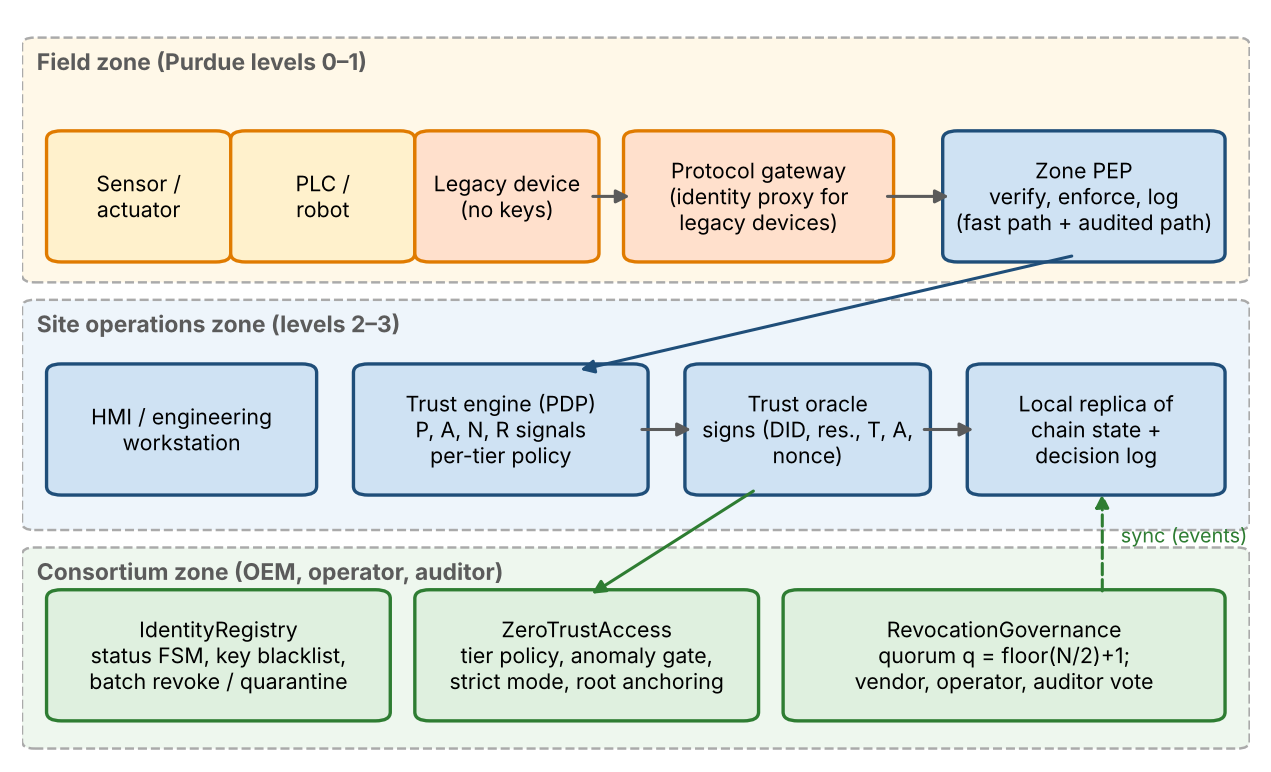
\includegraphics[width=0.62\textwidth]{../figures/fig7_iiot_arch.png}
\caption{Architecture of the blockchain-enabled Zero Trust system for Industrial IoT identity management, organized by plant zone.}
\label{fig:arch}
\end{figure*}

\subsection{Identity Lifecycle and the Registry}\label{sec:identity}
A device derives a DID from its public key in the style of the W3C data model \cite{w3cdid2022}, $\mathrm{did}=\texttt{did:iot:}\,\mathrm{H}(pk)[0{:}32]$, with SHA-256 in the testbed and Keccak-256 in the Solidity track. Commissioning submits $pk$ (or its hash), a device class, and a hash of the declared attributes (firmware version, vendor, location), signed by $sk$ so that the record proves key possession without exposing the attributes. The registry is a state machine:
\[
\text{UNKNOWN} \xrightarrow{\text{register}} \text{ACTIVE}
\]
\[
\text{ACTIVE} \xrightarrow{\text{suspend}} \text{SUSPENDED} \xrightarrow{\text{reinstate}} \text{ACTIVE}
\]
\[
\text{ACTIVE or SUSPENDED} \xrightarrow{\text{revoke}} \text{REVOKED (terminal)}
\]
REVOKED is terminal, and revocation also blacklists the key hash, so the same key cannot be enrolled under a new DID. Suspension is the reversible quarantine used while an advisory is assessed. All transitions are restricted to the registrar role and emit indexed events, which zone replicas and security monitoring consume.

\subsection{Legacy Devices Behind a Protocol Gateway}\label{sec:legacy}
Brownfield equipment often cannot sign requests. We represent each such device by a DID derived from the \emph{gateway's} key and the device's local address, registered with the class \texttt{legacy}. The gateway signs on its behalf and supplies weaker posture evidence (the testbed draws legacy posture from a lower range than native devices). Two rules keep this from lowering the security of the whole plant: the class check admits \texttt{legacy} identities only to low-consequence resources (tiers T0--T1 in our policy), and revoking the gateway key revokes every proxied identity at once. The trade-off is explicit: a compromised gateway can speak for every legacy device behind it, which is why this class never reaches the strict tiers.

\subsection{Tiered Zero Trust Policy}\label{sec:tiers}
Each resource has a policy $\pi=(\theta,m,g,s,\mathcal{C},\tau_{\max})$: a minimum trust $\theta$, a step-up margin $m$, an anomaly hard gate $g$, a strict flag $s$, a set of permitted device classes $\mathcal{C}$ and a maximum idle time $\tau_{\max}$. Table~\ref{tab:tiers} lists the four tiers used in our evaluation. The parameters are illustrative and tuned by hand to our synthetic signal ranges; a real plant would set them from its own telemetry and risk assessment.

\begin{table}[t]
\centering
\caption{Criticality tiers used in the evaluation}
\label{tab:tiers}
\scriptsize
\begin{tabular}{@{}llcccl@{}}
\toprule
\textbf{Tier} & \textbf{Example resource} & $\theta$ & $m$ & $g$ & \textbf{Classes} \\
\midrule
T0 & telemetry.read & 0.50 & 0.10 & 1.00 & all, incl.\ legacy \\
T1 & historian.write & 0.55 & 0.10 & 0.60 & all but HMI \\
T2 & plc.setpoint.write$^{\dagger}$ & 0.70 & 0.05 & 0.30 & HMI, PLC, robot \\
T3 & plc.firmware.update$^{\dagger}$ & 0.78 & 0.04 & 0.20 & PLC, robot \\
\bottomrule
\multicolumn{6}{l}{$^{\dagger}$ strict: borderline scores are denied rather than stepped up.}
\end{tabular}
\end{table}

The trust score combines four signals in $[0,1]$: device posture $P$ (attested firmware and configuration state), behavioural anomaly $A$, network context $N$ and historical reliability $R$ (mean of the last ten scores, 0.6 for a new device),
\begin{equation}
T=w_pP+w_b(1-A)+w_nN+w_rR,\label{eq:score}
\end{equation}
with default weights $(w_p,w_b,w_n,w_r)=(0.30,0.30,0.20,0.20)$,
\label{sec:signals}The signals come from the PEP and from monitoring that the plant already operates; in practice $A$ could be produced by process-aware anomaly detection, possibly trained across sites without sharing raw data \cite{tom2025flcti}. We treat their production as an input and evaluate only how the policy handles them. The oracle signs $(\mathrm{did},\mathrm{res},T,A,\mathrm{nonce})$; including $A$ in the signed message is what lets a contract enforce the gate without trusting the device's own report.

\begin{center}
\begin{minipage}{\linewidth}
\small
\textbf{Algorithm 1} \texttt{evaluateAccess(did, res, class, T, A, nonce, sig)}
\begin{enumerate}[leftmargin=1.4em,itemsep=0pt,topsep=2pt]
  \item \textbf{if} status(did) $\ne$ ACTIVE \textbf{or} no policy for res \textbf{then return} DENY
  \item \textbf{if} (did, nonce) already used \textbf{then return} DENY; mark it used
  \item \textbf{if} class $\notin\mathcal{C}$ \textbf{then return} DENY
  \item \textbf{if} oracle signature over (did, res, $T$, $A$, nonce) is invalid \textbf{then return} DENY
  \item \textbf{if} $A>g$ \textbf{then return} DENY \hfill\textit{(anomaly gate)}
  \item \textbf{if} $T<\theta$ \textbf{then return} DENY
  \item \textbf{if} $T<\theta+m$ \textbf{then return} (\textbf{if} strict \textbf{then} DENY \textbf{else} STEP\_UP)
  \item \textbf{return} ALLOW
\end{enumerate}
\end{minipage}
\end{center}

The gate and the strict flag address a specific weakness of weighted scores that Proposition~\ref{prop:bound} makes precise: because the score is linear, an attacker who spoofs posture, network and reliability can hold $T$ high no matter how abnormal its behaviour is, so for consequential resources the anomaly signal must be able to veto independently of the sum. For a step-up, we leave the second-factor mechanism to the plant (for example a local operator confirmation); STEP\_UP is never returned for strict resources.

\subsection{Hybrid Enforcement: Fast Path and Audited Path}\label{sec:hybrid}
Running Algorithm~1 on the chain for every request would cap throughput at what a block can carry and would couple plant operations to consensus latency. We therefore split enforcement by tier.
\begin{itemize}[leftmargin=1.1em,itemsep=0pt,topsep=1pt]
  \item \textbf{Fast path (T0, T1).} The zone PEP decides locally against its replica: status and key from the registry events, a per-device monotonic counter in place of the nonce set, the device's request signature, the oracle's attestation and the tier policy. Each decision appends a leaf to a log; every $B$ decisions the PEP computes a Merkle root and anchors it with \texttt{anchorDecisions(root, count)}, which only authorized PEP addresses may call. An auditor can later check any single logged decision against the anchored root.
  \item \textbf{Audited path (T2, T3).} The request is decided by \texttt{evaluateAccess} on the chain, so the decision, its inputs and its outcome are themselves on the ledger. These resources are written rarely and under operator control, which is what makes the cost acceptable; if a plant's setpoint writes are frequent, this assumption fails and the tiers must be re-cut.
\end{itemize}
The price of the fast path is the replica lag $\Delta$ of assumption A5: a device revoked just before a request may still be accepted for tier T0--T1 resources until the replica catches up (Proposition~\ref{prop:stale}). The audited path has no such window.

\subsection{Firmware Recall and Quarantine}\label{sec:recall}
When a vulnerability is disclosed in a firmware generation, the manufacturer needs to withdraw every affected device quickly. \texttt{revokeBatch(dids, reason)} revokes many devices in one transaction, skips unknown or already-revoked entries rather than reverting (so one stale entry cannot block a recall), blacklists each key and emits one event per device; \texttt{suspendBatch} quarantines them reversibly. The batch is limited by the block gas limit, and Section~\ref{sec:recall_eval} measures its per-device gas and the number of blocks needed for fleets of $10^3$--$5\times10^4$ devices.

\subsection{Decentralized Revocation Governance}\label{sec:governance}
A single registrar can deny service to legitimate devices, or reinstate a dangerous one. \texttt{RevocationGovernance} mediates \texttt{revokeDevice()} through threshold voting among $N$ independent voters, in the spirit of the voter group of \cite{kumar2026privacy}. A voter calls \texttt{propose(did, reason)}; each voter casts one \texttt{castVote(id, approve)}. The proposal executes the revocation as soon as approvals reach $q=\lfloor N/2\rfloor+1$, and is finalized as rejected once denials exceed $N-q$. The governance contract holds the registrar role on the registry; time-critical actions that a signed vendor bulletin pre-authorizes may use the direct path, so the two paths coexist. Votes are non-transferable, one per voter, and DENY votes never count toward approval.

\subsection{Degraded Operation During an Outage}\label{sec:outage}
If a PEP loses its replica feed, it must pick between availability and safety. Our policy is tier-dependent: T0--T1 requests continue against the last known state (accepting that a device revoked during the outage is not yet known), while audited-path requests (T2--T3) are \emph{denied}, because their decision needs the chain. This is fail-closed for consequential writes and fail-operational for reads; whether an operator accepts that trade is a plant decision, and Section~\ref{sec:outage_eval} quantifies it for a simple scenario.

\section{Security Analysis}\label{sec:security}
The contracts are deterministic state machines, so the proofs are short; they establish that the logic meets goals G1--G7 under A1--A5, not that a deployment is secure.

\subsection{Security Properties}\label{sec:props}
\begin{proposition}[Immediate revocation on the audited path, G1]\label{prop:revoke}
If \texttt{revokeDevice(did)} (or \texttt{revokeBatch} containing \texttt{did}) is in a finalized block, every later call to \texttt{evaluateAccess} for \texttt{did} returns DENY.
\end{proposition}
\emph{Proof.} By A1 the call sees finalized state with $\mathrm{status}(\mathrm{did})=$ REVOKED. No function leaves REVOKED, and step~1 of Algorithm~1 runs before every other check and denies all non-ACTIVE statuses. \hfill$\square$

\begin{proposition}[Bounded exposure on the fast path, G1]\label{prop:stale}
Let a revocation finalize at time $t_f$ and let a PEP satisfy A5. A fast-path request evaluated at time $\tau\ge t_f+\Delta$ is denied. If the device submits at most $\rho$ accepted requests per second, at most $\rho\Delta$ requests are accepted after $t_f$.
\end{proposition}
\emph{Proof.} By A5 the replica shows status REVOKED from $t_f+\Delta$ on, and the fast path denies non-ACTIVE devices before any other check. Requests accepted after $t_f$ therefore fall in $[t_f,t_f+\Delta)$, which holds at most $\rho\Delta$ of them. \hfill$\square$

\begin{proposition}[Replay resistance, G2]\label{prop:replay}
For a single PEP and any $(\mathrm{did},c)$ with $c$ a nonce (audited) or counter value (fast path), at most one evaluation returns ALLOW or STEP\_UP.
\end{proposition}
\emph{Proof.} Audited path: the test-and-set of the used-nonce flag is one transaction and transactions execute serially, so a second evaluation sees the flag and denies at step~2. Fast path: the PEP accepts only counters greater than the stored maximum and then stores the new value, so a repeated or older counter is denied. In a multi-PEP zone, the PEP identity must be bound into the signed message so that a request captured at one PEP is useless at another; our testbed exercises a single PEP. \hfill$\square$

\begin{proposition}[Attestation unforgeability, G3]\label{prop:oracle}
A PPT adversary without $sk_\mathcal{O}$ obtains ALLOW or STEP\_UP for a pair $(T,A)$ not attested by $\mathcal{O}$ for that request only with negligible probability.
\end{proposition}
\emph{Proof.} Steps 5--8 are reached only after the signature over $(\mathrm{did},\mathrm{res},T,A,\mathrm{nonce})$ verifies under $pk_\mathcal{O}$. Producing a different $(T,A)$ with a valid signature is an EUF-CMA forgery (A2). The nonce is inside the message, so an attestation cannot be moved to another request. Changing only $A$ (for example, reporting a lower anomaly) changes the signed message, which the contract tests demonstrate. \hfill$\square$

\begin{proposition}[Key-reuse prevention, G4]\label{prop:key}
After a finalized revocation, \texttt{registerDevice} with the same key hash reverts.
\end{proposition}
\emph{Proof.} Revocation sets $\mathrm{revokedKey}[\mathrm{H}(pk)]$, and registration reverts on that flag. Since the DID is a function of $\mathrm{H}(pk)$, a new identity needs a new key, which the adversary lacks unless it compromised another device. \hfill$\square$

\begin{proposition}[Governance safety and liveness, G6]\label{prop:gov}
With $N$ voters and quorum $q$: (a) a revocation executes only if at least $q$ distinct voters approved; (b) a set of at most $N-q$ voters cannot stop a proposal that the other $q$ approve; (c) a coalition of at most $q-1$ voters cannot execute a revocation.
\end{proposition}
\emph{Proof.} (a) \texttt{hasVoted} blocks repeats and \texttt{isVoter} blocks outsiders; the approval counter reaches $q$ only with $q$ distinct approvals, and only then is \texttt{revokeDevice} called. (b) Denials end a proposal only when they exceed $N-q$, which at most $N-q$ dissenters cannot, so the $q$ approvers can always complete. (c) Fewer than $q$ approvals never trigger execution. Safety additionally requires that no other registrar path exists for the affected devices. \hfill$\square$

\begin{proposition}[Spoofing, the gate and strictness, G5]\label{prop:bound}
(a) If scores $T,T'$ differ only in signal $s_j$ with weight $w_j$, then $|T-T'|\le w_j$. (b) On a resource with gate $g$, every ALLOW satisfies $A\le g$. (c) On a strict resource, every ALLOW satisfies $T\ge\theta+m$. (d) For an attacker with $P=N=R=1$, $T=1-w_bA$, and it is accepted on a strict resource if and only if $A\le\min\{g,(1-\theta-m)/w_b\}$.
\end{proposition}
\emph{Proof.} (a) $T-T'=w_j(s_j-s_j')$ and $|s_j-s_j'|\le1$. (b) and (c) are steps 5 and 7 of Algorithm~1. (d) Substituting gives $T=0.3+0.3(1-A)+0.2+0.2=1-0.3A$, and ALLOW needs $A\le g$ and $T\ge\theta+m$. \hfill$\square$

\emph{Corollary (what a fixed threshold cannot do).} With the default weights a fully spoofing attacker has $T\ge0.70$ even at $A=1$. Hence on a non-strict resource with $\theta=0.55$ and no gate, \emph{no} anomaly value gets such an attacker denied, and for the tiers of Table~\ref{tab:tiers} the bound $(1-\theta-m)/w_b$ is $0.83$ (T2) and $0.60$ (T3), above the gates $0.30$ and $0.20$; the \emph{gate}, not the score, is what stops the attacker, and the residual risk is exactly the set of attackers who keep $A\le g$. The experiments of Section~\ref{sec:gate_eval} measure how that residual behaves.

\subsection{Residual Risks}\label{sec:residual}
The properties say nothing about (i) compromised validators or oracle keys (A1, A4); (ii) a stolen key used by an attacker who behaves like the owner until revoked, which no continuous scheme separates from the owner except by behaviour; (iii) side-channel extraction of keys; or (iv) smart-contract defects, for which the quality-assurance literature recommends testing, verification and audit \cite{wei2024quality}. Also, the trust oracle is a trusted data source, which is the blockchain-oracle problem in a specific form \cite{hassan2023oracle}; a threshold-signed oracle would reduce it (Section~\ref{sec:disc}). Finally, the nonce set costs one storage slot per accepted audited request and needs epoch-based pruning in a long-lived deployment.

\section{Prototype Implementation}\label{sec:impl}

\subsection{Two Tracks}\label{sec:env}
\textbf{Track A -- Solidity on an EVM.} \texttt{IdentityRegistry.sol}, \texttt{ZeroTrustAccess.sol} and \texttt{RevocationGovernance.sol} (Solidity 0.8.24, optimizer 200 runs) implement Section~\ref{sec:arch}: the status machine, Algorithm~1 with anomaly gate and strict mode, \texttt{revokeBatch}/\texttt{suspendBatch}, PEP-authorized root anchoring, and quorum voting. They are compiled with solc-js and executed on the Hardhat in-process EVM. A Mocha/Chai suite of 13 tests passes; besides the registry, replay, revocation and governance cases it covers the industrial additions: the gate denies a high composite score when $A>g$, a tampered anomaly value invalidates the oracle signature, strict resources never step up, batch revocation skips unknown entries and blocks later access, and only authorized PEPs can anchor. Scripts measure gas for every operation. This track gives real gas but, on its own, not multi-node consensus or network latency (Track C adds those), and the device's request signature is verified by the PEP rather than on-chain.

\textbf{Track B -- Python testbed.} A Python implementation of the same state machine uses real Ed25519 (the \texttt{cryptography} library), SHA-256 and a Merkle root. Besides the contract model it contains the \texttt{FastPathPEP}, which verifies the device signature and the oracle attestation (two Ed25519 verifications), applies the per-device counter and tier policy, and logs decisions in Merkle-rooted batches. It is used for scale, statistical, baseline, tier and governance experiments. The host is a 2-vCPU Linux container (Python 3.13, Hardhat 2.22); all seeds derive from 20261004. Track B uses Ed25519 whereas Track A uses secp256k1 ECDSA, so their timings are not comparable.

\textbf{Track C -- Four-validator QBFT network.} The same contracts are deployed on Hyperledger Besu 25.7.0 with four validators (QBFT, 2\,s block period, 4\,s round timeout, chain ID 2026, zero base fee, one JVM of 700\,MB per node, ports 8545--8548) started by \texttt{start\_net.sh} from \texttt{qbftConfigFile.json}. \texttt{besu\_benchmark.js} (ethers v6) measures block interval, sequential call latency, revocation visibility on a second validator, throughput with pre-signed transactions from ten senders, quorum voting and batch recall, and \texttt{besu\_fault.js} stops and restarts validators. Everything, including the load generator, shares the same two-vCPU host, which limits the throughput results (Section~\ref{sec:besu_eval}).

\subsection{Industrial Fleet and Signal Model}\label{sec:devsim}
The synthetic fleet has six classes with proportions sensor 40\%, PLC 15\%, HMI 8\%, robot 7\%, gateway 15\% and legacy 15\%. Native devices draw posture in $[0.75,1]$, anomaly in $[0,0.15]$ and network context in $[0.7,1]$; legacy devices draw posture in $[0.55,0.75]$, anomaly in $[0,0.20]$ and network in $[0.6,0.9]$. To mimic process upsets, a fraction of legitimate requests (5\% by default; 0, 5 and 15\% in the sensitivity study) draws anomaly from $[0.15,0.45]$. Four attack populations are used: \emph{naive compromise} (all signals degraded), \emph{partial mimicry} (posture and network legitimate, $A\in[0.3,0.7]$), \emph{stealthy mimicry} ($A\in[0.15,0.40]$) and \emph{full spoof} ($P=N=1$, $A\in[0.3,0.7]$); each starts from three clean prior requests. The legacy gateway of Section~\ref{sec:legacy} is modelled through the class \texttt{legacy} and its weaker signals; deriving proxy DIDs from the gateway key is a design element we did not implement. In the synthetic experiments the distributions are our assumptions, not field measurements, and the attack and legitimate ranges overlap by construction, so they show how the policy responds to such overlap rather than how well a detector would perform in a plant. The real-data experiment of Section~\ref{sec:real_eval} (\texttt{sim/experiments\_realdata.py}, scikit-learn 1.9) replaces only the behavioural signal.

\subsection{Experiment Scenarios and Reproducibility}\label{sec:scenarios}
\emph{Carried over from the base design:} (S1) scaling over $n\in\{50,\dots,1600\}$; (S2) 500 trials per basic attack; (S3) 30 repeated runs at $n=400$; (S4) baseline revocation exposure for 60 devices at 1 request/s over 600 logical seconds with revocation times from $U(100,500)$\,s; (S5) governance with 200 trials per $N\in\{5,\dots,21\}$ under cooperation, maximal dissent and forced revocation; and a trust-signal ablation. \emph{Industrial additions:} (X1) tiered policy on the mixed fleet, 4{,}000 requests per population; (X2) anomaly-gate sweep; (X3) fast path versus modelled on-chain path, 10 runs of 2{,}000 requests over 300 PLC and robot devices; (X4) recall capacity from measured gas; and (X5) outage scenario; and (R) the TON\_IoT study of Section~\ref{sec:real_eval}, with five seeds for detector quality and one seed for held-out types and the policy runs. The commands are \texttt{python -m sim.benchmark}, \texttt{sim.experiments\_extra}, \texttt{sim.experiments\_governance}, \texttt{sim.experiments\_iiot}, \texttt{sim.experiments\_realdata} (needs the TON\_IoT CSVs in \texttt{data/}; they are not redistributed) and \texttt{hardhat run scripts/measure\_gas.js}, \texttt{measure\_governance\_gas.js}, \texttt{measure\_iiot\_gas.js}; \texttt{paper/gen\_tables.py} regenerates every table from the resulting JSON files.

\section{Experimental Evaluation}\label{sec:eval}

\subsection{Methodology and What the Numbers Mean}\label{sec:metrics}
We report decision latency and throughput, on-chain gas, revocation exposure (requests accepted after the revocation instant), per-tier acceptance of legitimate and attacking requests, quorum behaviour, recall capacity and a degraded-mode scenario. Latencies are wall-clock times from a monotonic timer. Three limits apply throughout. (i) Testbed numbers are \emph{compute-bound}: they exclude network, block time and multi-node consensus. (ii) Sections~\ref{sec:scaling}--\ref{sec:outage_eval} use \emph{synthetic} devices, signals and attacks, so their detection-type results characterize policy mechanics under stated overlaps; Section~\ref{sec:real_eval} replaces the behavioural signal with detector scores computed on real TON\_IoT traffic, while posture and network context remain synthetic. (iii) One two-vCPU host was used.

\subsection{Testbed Performance and Repeated-Run Statistics}\label{sec:scaling}
Table~\ref{tab:results} gives one run per fleet size. Mean authorization latency is 0.120--0.197\,ms and registration 0.173--0.286\,ms; the two smallest fleets are slower (0.184 and 0.197\,ms against 0.120--0.127\,ms for $n\ge200$), probably from warm-up, which we did not isolate. Beyond $n=200$ latency is flat as the fleet grows eightfold, consistent with constant per-request cost dominated by one Ed25519 verification. Throughput is 3{,}700--6{,}200 decisions/s. Repeating $n=400$ thirty times gives a mean authorization latency of $0.133\pm0.013$\,ms (95\% CI 0.128--0.138) and registration $0.184\pm0.019$\,ms; over 20{,}000 sequential decisions the percentiles are p50 0.124, p95 0.188, p99 0.247 and p99.9 0.932\,ms, with a 4.3\,ms maximum attributable to scheduling or garbage collection. Intervals assume roughly normal run means and apply to this host.

\begin{table}[t]
\centering
\caption{Scaling results, one run per fleet size (latency in ms, throughput in ops/s)}
\label{tab:results}
\scriptsize
\begin{tabular}{@{}rrrrrr@{}}
\toprule
$n$ & Reg.\ lat. & AuthZ lat. & AuthZ p95 & Reg.\ tput & AuthZ tput \\
\midrule
50 & 0.286 & 0.184 & 0.216 & 3{,}477 & 3{,}812 \\
100 & 0.282 & 0.197 & 0.236 & 3{,}539 & 3{,}679 \\
200 & 0.256 & 0.125 & 0.148 & 3{,}906 & 5{,}909 \\
400 & 0.173 & 0.120 & 0.143 & 5{,}755 & 6{,}159 \\
800 & 0.177 & 0.127 & 0.162 & 5{,}645 & 5{,}804 \\
1{,}600 & 0.175 & 0.126 & 0.153 & 5{,}693 & 5{,}879 \\
\bottomrule
\end{tabular}
\end{table}

\subsection{On-Chain Cost: Measured EVM Gas}\label{sec:gas}
Table~\ref{tab:gas} lists gas measured over 50 devices on the Hardhat EVM; gas is deterministic given the state path (s.d.\ below 10). Registration costs about 215k gas and a full audited decision about 70k, of which one \texttt{ecrecover} and one new nonce slot are the main parts. Requests denied for replay (41.5k) or against a revoked device (39.3k) are cheaper because they exit early, while denials that occur after the oracle check cost as much as an allow. The industrial additions cost nothing visible: an ALLOW on a strict resource (70.4k), an anomaly-gate denial (70.2k), a strict-borderline denial (70.4k) and a below-threshold denial (70.2k) are all within 0.3\% of the base decision, since the extra checks are cheap comparisons. Anchoring a decision-log root costs 70.8k gas for the first anchor and 53.7k in steady state, which is 54 gas per decision at $B=1000$ decisions per root, about three orders of magnitude below the 70.4k of deciding each of them on-chain.

\begin{table}[t]
\centering
\caption{Measured gas per operation (Hardhat EVM, solc 0.8.24, 50 devices)}
\label{tab:gas}
\scriptsize
\begin{tabular}{@{}lrr@{}}
\toprule
\textbf{Operation} & \textbf{Mean gas} & \textbf{Std.} \\
\midrule
\texttt{registerDevice} & 214{,}950 & 8.9 \\
\texttt{suspendDevice} & 32{,}709 & 5.9 \\
\texttt{reinstateDevice} & 32{,}901 & 5.9 \\
\texttt{revokeDevice} & 58{,}824 & 5.9 \\
\texttt{evaluateAccess} (ALLOW) & 70{,}368 & 9.7 \\
\texttt{evaluateAccess} (STEP\_UP) & 70{,}413 & 8.0 \\
\texttt{evaluateAccess} (DENY, bad oracle sig.) & 70{,}143 & 8.3 \\
\texttt{evaluateAccess} (DENY, replay) & 41{,}526 & 9.7 \\
\texttt{evaluateAccess} (DENY, revoked) & 39{,}308 & 8.4 \\
\midrule
Deploy \texttt{IdentityRegistry} & 1{,}333{,}022 & -- \\
Deploy \texttt{ZeroTrustAccess} & 1{,}079{,}680 & -- \\
\texttt{definePolicy} (2 classes) & 97{,}805 & -- \\
\bottomrule
\end{tabular}
\end{table}

For capacity planning, a 30M-gas block (a typical default; PoA operators choose their own) holds at most $\lfloor 30\text{M}/70{,}369\rfloor=426$ audited decisions or 139 registrations. This is a gas-based upper bound, not a measured throughput (Section~\ref{sec:besu_eval} measures a much lower sustained rate on a real network), and it is the reason why only T2--T3 are decided on-chain. The in-process call latency including client-side signing was about 3\,ms per decision, an upper bound on pure EVM execution that says nothing about network or consensus delay.

\subsection{Hybrid Enforcement: Cost of the Fast Path}\label{sec:fast_eval}
We compare the contract model, which verifies one signature per decision (Track B), with the fast-path PEP, which verifies the device signature and the oracle attestation. Over 10 runs of 2{,}000 mixed T0/T2 requests, the contract model takes $0.134\pm0.020$\,ms (95\% CI 0.119--0.148) and the fast path $0.261\pm0.022$\,ms (CI 0.245--0.277). The fast path is therefore about twice as expensive \emph{in compute}, which is the expected cost of two verifications; it sustains roughly 3{,}800 decisions/s on one core. Its benefit is elsewhere: it needs no transaction, no gas and no block, and it keeps working when the ledger is slow. The compute comparison is thus a cost, not a gain, and the real advantage depends on the network and consensus latency that we did not measure.

\subsection{Tiered Policy: Legitimate Acceptance and Attack Acceptance}\label{sec:tiers_eval}
Table~\ref{tab:tiersres} runs 4{,}000 legitimate requests (5\% with a process upset) and 4{,}000 requests of each attack population through the four tiers, first with threshold alone and then with the full policy (gate and strict mode); eligibility is by device class, so the legitimate denominators shrink with the tier (4{,}000, 3{,}713, 1{,}145, 858). Fig.~\ref{fig:iiotres}(a) shows the same data graphically.

\begin{table}[t]
\centering
\caption{Per-tier results: legitimate requests allowed and attacker requests accepted (\%), threshold alone $\to$ full policy ($\theta$ min.\ trust, $g$ anomaly gate)}
\label{tab:tiersres}
\scriptsize
\setlength{\tabcolsep}{2.2pt}
\begin{tabular}{@{}lccrrr@{}}
\toprule
\textbf{Resource} & $\theta$ & $g$ & Legit. & Stealthy & Spoof \\
\midrule
telemetry.read (T0) & 0.50 & 1.00 & 100.0$\to$100.0 & 100.0$\to$100.0 & 100.0$\to$100.0 \\
historian.write (T1) & 0.55 & 0.60 & 100.0$\to$100.0 & 100.0$\to$100.0 & 100.0$\to$74.7 \\
plc.setpoint.write (T2) & 0.70 & 0.30 & 99.9$\to$97.8 & 98.5$\to$60.9 & 100.0$\to$0.0 \\
plc.firmware.update (T3) & 0.78 & 0.20 & 96.0$\to$94.8 & 52.2$\to$13.6 & 52.4$\to$0.0 \\
\bottomrule
\end{tabular}
\end{table}

Four observations follow. First, naive compromise is denied everywhere (0\% accepted at all tiers), so it does not test the design. Second, at T0 an attacker that spoofs signals is accepted 100\% of the time under any policy: this is by design, since T0 is read-only telemetry and we chose not to spend verification effort there, but it means T0 data can be read by a compromised device that keeps looking normal. Third, the gate and strict mode matter exactly where consequences are high: at T2 the full-spoof attacker falls from 100\% to 0\% accepted and the stealthy attacker from 98.5\% to 60.9\%; at T3 from 52.4\% to 0\% and from 52.2\% to 13.6\%. Fourth, this has a price. Legitimate allowance drops from 99.9\% to 97.8\% at T2 and from 96.0\% to 94.8\% at T3 (and 5.2\% of legitimate T3 requests are denied outright), because upset requests exceed the gate and strict mode refuses borderline scores. A plant would decide whether those denials are acceptable for setpoint and firmware writes, where a second confirmation is usually welcome, and the next experiment shows the trade-off.

A short ablation of the trust signals, run in the base design, adds that the full score separates partial and stealthy mimicry with AUC 0.993 and 0.895 whereas dropping the behavioural signal leaves both at AUC 0.499--0.500, so the behavioural signal is the only one that separates mimicry from legitimate traffic in this setup; posture and network are drawn from the same ranges for both populations in the synthetic fleet, so removing them \emph{raises} AUC, which argues for adaptive rather than fixed weighting and should not be read as evidence that real posture is uninformative.

\subsection{Sensitivity to the Anomaly Gate}\label{sec:gate_eval}
Fig.~\ref{fig:iiotres}(b) sweeps the gate level from 0.15 to 0.60 for legitimate upset rates of 5\% and 15\% (0\% gives no false denials by construction). Under a 5\% upset rate, a gate of 0.30 blocks 40.1\% of stealthy mimicry and 100\% of full spoofing while denying 2.3\% of legitimate requests. Tightening to 0.25 and 0.20 raises the stealthy block rate to 60.4\% and 80.4\% at 3.1\% and 3.8\% legitimate denials, and 0.15 blocks all of it at 4.6\%. Loosening to 0.40 blocks no stealthy attacker and lets 25\% of full spoofing through, rising to 74\% at 0.60. At a 15\% upset rate the same gates deny 7.4\% (0.30) and 12.2\% (0.20) of legitimate requests. The gate is thus a genuine trade-off whose operating point depends on how noisy legitimate behaviour is, and because the attack range $[0.15,0.40]$ is built to overlap legitimate upsets, no gate separates them completely; an attacker who keeps its anomaly below the gate is accepted, as Proposition~\ref{prop:bound}(d) predicts.

\subsection{Evaluation on Real Traffic: TON\_IoT}\label{sec:real_eval}
The synthetic study fixes the anomaly distributions by hand, so we repeat the central experiments with the anomaly signal $A$ produced by detectors on a public dataset. We use the TON\_IoT collection, which provides labelled IIoT telemetry \cite{alsaedi2020ton} and labelled network flows \cite{moustafa2021network}; the heterogeneity of its features and attack types is analysed in \cite{booij2022ton}. The dataset licence grants free use for academic research on condition that the dataset papers are cited. We used four telemetry files (Fridge, Modbus, Thermostat, Weather) and the network file (211{,}043 flows, of which 190{,}474 remain after removing 20{,}569 exact duplicates; nine attack types plus normal traffic).

\emph{Method.} Features exclude IP addresses and source ports, and for telemetry exclude dates and times, because normal and attack records were collected on different days. A gradient-boosted classifier (supervised) and an Isolation Forest trained on normal records only (unsupervised) are evaluated on a stratified 70/30 split repeated over five seeds. To approximate attacks unseen at training time, we also train the classifier with one attack type left out and score that type (seed 11). The classifier's attack probability is used as $A\in[0,1]$. Legitimate requests carry the score of a normal test flow, attackers carry the score of an attack flow and spoof posture and network context to 1 (the full-spoof attacker of Section~\ref{sec:devsim}); posture, network context and the reliability warm-up stay synthetic, and because the files share no device identifier, assigning a flow-derived score to a device is arbitrary. The four tiers of Table~\ref{tab:tiers} are used unchanged.

\emph{Telemetry alone is a weak signal.} Table~\ref{tab:telemetry} shows that only the Weather file separates attacks from normal records usefully (supervised AUC 0.972, Isolation Forest 0.819); Modbus gives 0.623 and 0.498, and Thermostat and Fridge are close to chance (0.513 and 0.531 supervised). The Fridge result requires a warning: before whitespace stripping, one column (\texttt{temp\_condition}) carries label-specific padding that gives a perfect AUC of 1.0, an encoding artefact that has nothing to do with device behaviour, so we strip all strings before training. We did not investigate why most telemetry is uninformative; one plausible reading is that the attacks target the services around a device rather than the physical readings it reports. The practical consequence is that a behavioural signal for a plant should come from traffic, not only from sensor values.

\begin{table}[t]
\centering
\caption{Detectability of attacks from TON\_IoT telemetry (five seeds, 70/30 split, after de-duplication)}
\label{tab:telemetry}
\scriptsize
\begin{tabular}{@{}lrrrr@{}}
\toprule
File & Rows & Att.\% & Sup. AUC & IF AUC \\
\midrule
Fridge & 37{,}110 & 67 & 0.531 & 0.484 \\
Modbus & 17{,}792 & 78 & 0.623 & 0.498 \\
Thermostat & 32{,}350 & 55 & 0.513 & 0.497 \\
Weather & 39{,}260 & 62 & 0.972 & 0.819 \\
\bottomrule
\end{tabular}
\end{table}

\emph{Network flows are a strong signal, with a caveat.} On flows the supervised classifier reaches AUC 0.9999 (s.d.\ below $10^{-4}$) and the Isolation Forest $0.916\pm0.004$, ranging from 0.813 (DDoS) to 0.956 (password attacks) by type. The near-perfect supervised value should be read as an upper bound: random splits of a benchmark whose attacks come from a few source hosts are optimistic, which is why we also test held-out types. With an attack type withheld, the AUC against normal traffic stays at 0.990--1.000, but the share of that type's flows scored above 0.5 falls to 65.4\% for ransomware and 73.7\% for man-in-the-middle, against 93--100\% for most others. Legitimate flows are overwhelmingly scored near zero (median 0.0003), but the tail is heavy: the 99th percentile is 0.27 and the 99.9th is 0.96, so any gate cuts into some legitimate traffic (see the gate sweep below).

\emph{Policy on real scores.} Table~\ref{tab:realpolicy} gives the percentage of attacker requests accepted, averaged over the nine attack types and, in the worst-case columns, for the single worst type, with threshold alone (Thr.) and with the full policy (gate and strict mode). Four findings follow. First, the full policy costs legitimate traffic little: allowance falls from 99.7, 99.5 and 99.0\% to 99.6, 98.8 and 98.4\% at T1, T2 and T3. Second, for attack types seen in training, the gate matters at T1 (mean acceptance 100\% $\to$ 0.7\%, worst 4.9\%, man-in-the-middle), whereas at T2 and T3 the high thresholds already reject nearly all such flows (1.1\% and 0.6\% with threshold alone), because a real detector scores them near 1 and Proposition~\ref{prop:bound}(d) then gives $T\approx0.7$ or below. This corrects the synthetic study, in which the stealthy population was built to sit at $A\le0.4$ and therefore overstated how often the threshold alone fails on seen attacks. Third, for held-out types, residual acceptance grows to 11.9\% (T1), 7.9\% (T2) and 6.6\% (T3) on average, and to 41.6\%, 33.9\% and 35.8\% for the worst type (ransomware), so a policy that depends on a detector inherits the detector's blind spots. Fourth, an adaptive attacker that can observe the detector and send only its best-scoring flows is much more dangerous: if it can send only the lowest-scoring 10\% of a held-out type's flows, mean acceptance at T1--T3 is 59.4, 37.9 and 29.0\%, and 76.5, 74.7 and 58.2\% for the best 1\%, with some types always accepted. We assume here that the attacker can query the detector and craft traffic with a chosen score, which is a strong capability, so these numbers describe a worst case rather than a typical one.

\begin{table}[t]
\centering
\caption{Attacker requests accepted (\%) with real TON\_IoT anomaly scores: mean over nine attack types and worst single type; threshold alone (Thr.) versus full policy}
\label{tab:realpolicy}
\scriptsize
\begin{tabular}{@{}llrrrr@{}}
\toprule
Scenario & Tier & Thr.\ mean & Full mean & Thr.\ worst & Full worst \\
\midrule
Seen types & T1 & 100.0 & 0.7 & 100.0 & 4.9 \\
 & T2 & 1.1 & 0.4 & 7.5 & 2.3 \\
 & T3 & 0.6 & 0.3 & 3.9 & 1.5 \\
\midrule
Held-out types & T1 & 100.0 & 11.9 & 100.0 & 41.6 \\
 & T2 & 15.9 & 7.9 & 51.5 & 33.9 \\
 & T3 & 9.3 & 6.6 & 36.7 & 35.8 \\
\midrule
Held-out, best 10\% & T1 & 100.0 & 59.4 & 100.0 & 100.0 \\
 & T2 & 64.1 & 37.9 & 100.0 & 100.0 \\
 & T3 & 49.3 & 29.0 & 100.0 & 100.0 \\
\midrule
Held-out, best 1\% & T1 & 100.0 & 76.5 & 100.0 & 100.0 \\
 & T2 & 87.4 & 74.7 & 100.0 & 100.0 \\
 & T3 & 76.0 & 58.2 & 100.0 & 100.0 \\
\bottomrule
\end{tabular}
\end{table}

Sweeping the gate on the real scores, a gate of 0.05 denies 3.6\% of legitimate flows and blocks 100\% of seen and 99.4\% of held-out attack flows; 0.30 denies 1.0\% and blocks 99.9\% and 94.6\%; 0.70 denies 0.3\% and blocks 99.7\% and 88.6\%; and 0.90 denies 0.2\% and blocks 99.5\% and 82.9\%. The real-score gate thus has a far better operating region than the synthetic one, because real attack scores are bimodal, but it degrades on unseen attack types. Detector hyper-parameters were left at library defaults, and the tier thresholds and gates are those fixed earlier for the synthetic study; none was tuned on these results.

\begin{figure*}[t]
\centering
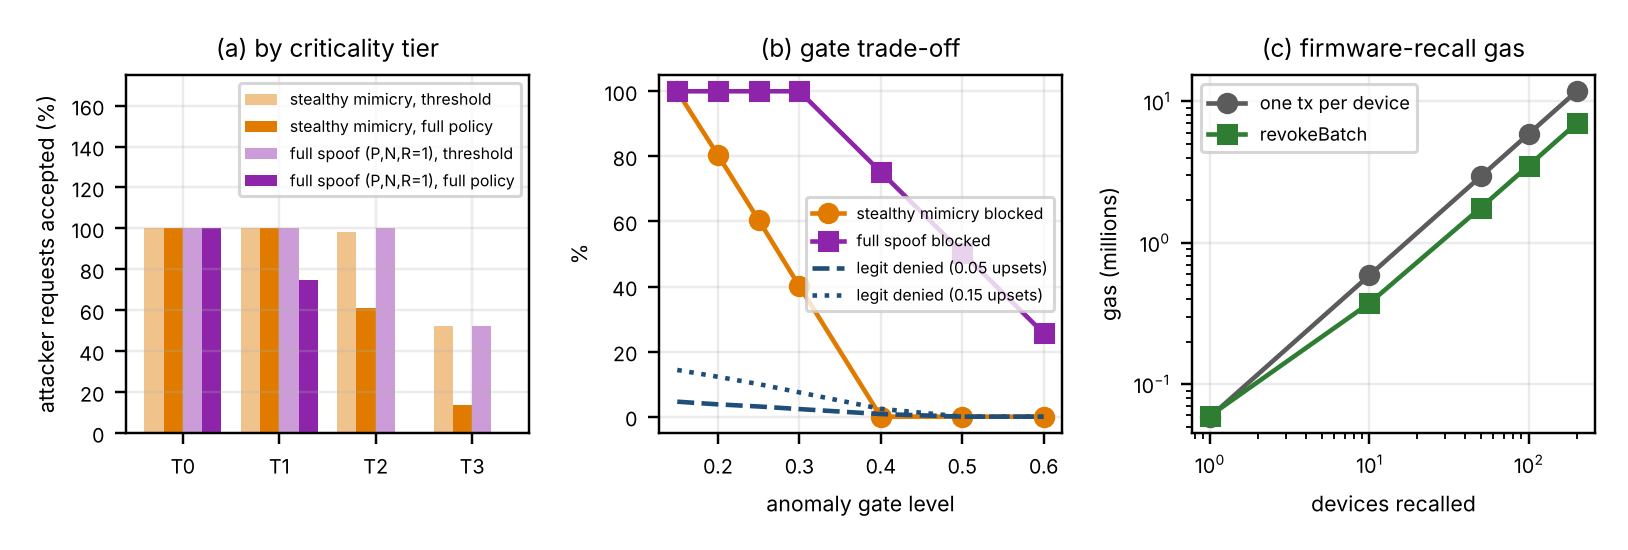
\includegraphics[width=0.86\textwidth]{../figures/fig8_iiot_results.png}
\caption{Industrial extensions: (a) attacker requests accepted per criticality tier under threshold-only and full policy; (b) anomaly-gate trade-off for 5\% and 15\% legitimate process-upset rates; (c) gas to recall devices with one transaction per device versus \texttt{revokeBatch}.}
\label{fig:iiotres}
\end{figure*}

\subsection{A Second Dataset: WUSTL-IIOT-2018 (SCADA)}\label{sec:wustl_eval}
To check that the gate behaviour is not specific to one collection, we repeat the policy experiment on WUSTL-IIOT-2018, flow records captured on a SCADA testbed with injected attacks \cite{teixeira2018scada,teixeira2018wustl}. The file has 7{,}037{,}983 rows and seven columns but only 62{,}959 distinct rows (99.1\% duplicates; 39{,}817 normal and 23{,}142 attack), and it carries a binary label only. Two consequences follow. First, de-duplication is essential: a random split of the raw file puts identical records in training and test data. Second, there are no attack types, so the held-out-type test of Section~\ref{sec:real_eval} cannot be repeated. We exclude the source port, as before, which leaves five count features (total, source and destination packets, total and source bytes), and use a stratified 70/30 split on the unique rows over five seeds.

A gradient-boosted classifier is almost perfect (AUC 0.99998, sd $2\times10^{-5}$): attack flows in this testbed are short (a median of two packets, at most 22) and normal flows are not, so the task is nearly trivial and the result says little about hard attacks. An Isolation Forest trained on normal flows only reaches AUC $0.909\pm0.006$, a more realistic stand-in for an attack never seen in training. For the policy we map the Isolation Forest score to $A\in[0,1]$ using normal training data alone (median to the 99.9th percentile), so no attack information enters the calibration.

Table~\ref{tab:wustl} gives the results. With the supervised score the full policy accepts at most 0.3\% of attack requests at T1--T3 and denies at most 0.2\% of legitimate ones, essentially the TON\_IoT picture. With the unsupervised score the gate and strict mode still reduce attack acceptance at the two critical tiers from 100\% and 94.1\% (threshold only) to 8.2\% and 4.3\%, but legitimate allowance drops to 87.5\% at T2 and 82.2\% at T3, a cost far above the 1--2\% seen with the supervised detector, because many normal flows look unusual to a detector fitted on five coarse counters. At T0 and T1 the unsupervised variant accepts all attack requests: the T1 gate is 0.60, above the median attack score of about 0.49. For an adaptive attacker that sends only its best 10\% (1\%) of flows, acceptance with the unsupervised score is 86.9\% (100\%) at T2 and 43.0\% (100\%) at T3, against 2.1\% (16.0\%) and 0.7\% (6.3\%) with the supervised score. A gate sweep with the unsupervised score shows the same trade-off as before: a gate of 0.3 denies 12.5\% of legitimate flows and blocks 91.3\% of attack flows, and a gate of 0.5 blocks none. The finding that carries over is the role of the gate; the finding that does not is that a strong detector is available. When the detector is weak, as an unsupervised one on coarse features is, the policy trades a large share of legitimate availability for protection at the critical tiers. As with TON\_IoT, posture and network context are synthetic and the flow-to-device pairing is arbitrary.

\begin{table}[t]
\centering
\caption{WUSTL-IIOT-2018: legitimate requests allowed and attack requests accepted (\%) under the threshold-only and full policies, for two sources of the anomaly signal}
\label{tab:wustl}
\scriptsize
\setlength{\tabcolsep}{2.5pt}
\begin{tabular}{@{}lrrrrrr@{}}
\toprule
 & \multicolumn{3}{c}{Supervised $A$} & \multicolumn{3}{c}{Isolation Forest $A$} \\
\cmidrule(lr){2-4}\cmidrule(lr){5-7}
Tier & Legit & Att.\ thr. & Att.\ full & Legit & Att.\ thr. & Att.\ full \\
\midrule
T0 & 100.0 & 100.0 & 100.0 & 99.3 & 100.0 & 100.0 \\
T1 & 100.0 & 100.0 & 0.1 & 97.1 & 100.0 & 100.0 \\
T2 & 100.0 & 0.3 & 0.3 & 87.5 & 100.0 & 8.2 \\
T3 & 99.8 & 0.2 & 0.1 & 82.2 & 94.1 & 4.3 \\
\bottomrule
\end{tabular}
\end{table}

\subsection{A Third Dataset With Attack Types: WUSTL-IIoT-2021}\label{sec:wustl21_eval}
WUSTL-IIoT-2021 contains Argus flow records from an industrial testbed running Modbus traffic, with four labelled attack types \cite{zolanvari2019vulnerability,zolanvari2021wustl}. It lets us repeat the held-out-type test that the SCADA file of Section~\ref{sec:wustl_eval} could not support. The file has 1{,}194{,}464 rows, 1{,}107{,}448 of them normal and the rest DoS (78{,}305), reconnaissance (8{,}240), command injection (259) and backdoor (212). All records were captured on one day, attacks come from two to four source hosts, and one column (\texttt{IdleTime}) is an epoch timestamp that separates attack types by capture time. We therefore drop timestamps, IP addresses, the source port, \texttt{IdleTime} and the IP-identification fields, keeping 39 features, and then remove 41{,}645 exact duplicates before splitting (1{,}152{,}819 rows remain). The evaluation follows Section~\ref{sec:real_eval}: a stratified 70/30 split over five seeds, a gradient-boosted classifier, an Isolation Forest trained on normal flows only (with $A$ calibrated on normal training scores alone, as before), and leave-one-type-out models as the held-out proxy.

\emph{Detection.} The supervised classifier is almost perfect on seen types (AUC 0.99999, and unchanged without the TTL fields, which fingerprint the attacker hosts). The Isolation Forest reaches AUC $0.987\pm0.001$, and between 0.983 and 0.990 for each attack type, because normal Modbus polling is very regular and the attacks (floods, scans) are far from it. Held-out detection is a different story: when DoS is removed from training, the classifier flags only 0.7\% of DoS test flows at 0.5 (AUC against normal 0.71), and for command injection and reconnaissance the figure is 8.1\% and 13.0\% although their AUC is above 0.999, which means the ranking is right but the scores sit far below any useful gate. Backdoor is found at 66.7\%. The command-injection and backdoor test sets contain only 74 and 63 flows, so those two figures are imprecise.

\emph{Policy.} Table~\ref{tab:wustl21} gives the full-policy results as means over the four attack types. With seen types the full policy admits 3.6--4.2\% of attack requests at T1--T3 (the average hides 10.8--12.1\% for backdoor and 3.8--4.5\% for command injection, the two rarest types) and denies none of the legitimate requests. With types withheld from training, acceptance rises to 75.4--77.8\% on average and to 97.9--99.2\% for DoS at the three higher tiers; the threshold-only policy is not much worse (last column), so on unseen types the supervised score contributes almost nothing, and an adaptive attacker sending its best 10\% or 1\% of flows is accepted in all cases. The unsupervised score behaves very differently on this data: the full policy admitted no attack request of any type at T1--T3, including the best 1\% of an adaptive attacker's flows, at the price of denying 1.5\%, 12.1\% and 22.3\% of legitimate requests at T1, T2 and T3. A gate of 0.5 on this score already blocks all attack flows while denying 2.3\% of legitimate ones, whereas the T2 and T3 gates (0.30 and 0.20) deny 12.0\% and 21.5\%. The two datasets with attack types therefore agree on the main point and disagree on the detector: a supervised detector does not protect against attack types it has not seen, and a detector trained on normal traffic only can, but only when normal traffic is as regular as it is in this testbed.

\emph{Limits of this result.} The favourable unsupervised numbers come from a laboratory testbed with machine-generated, nearly constant normal traffic and volumetric attacks from a handful of hosts, which makes anomaly detection easier than in a plant with operators, engineering workstations and maintenance windows. The rare attack types have very few flows, posture and network context are synthetic, and the pairing of a flow with a device is arbitrary.

\begin{table}[t]
\centering
\caption{WUSTL-IIoT-2021: legitimate requests allowed and attack requests accepted (\%) under the full policy, as means over four attack types; ``Thr.-only'' is the threshold-only policy on the held-out supervised scores}
\label{tab:wustl21}
\scriptsize
\setlength{\tabcolsep}{2.5pt}
\begin{tabular}{@{}lrrrrrr@{}}
\toprule
 & \multicolumn{3}{c}{Supervised $A$} & \multicolumn{2}{c}{Isolation Forest $A$} & \\
\cmidrule(lr){2-4}\cmidrule(lr){5-6}
Tier & Legit & Seen & Held-out & Legit & Attack & Thr.-only$^{a}$ \\
\midrule
T0 & 100.0 & 100.0 & 100.0 & 99.4 & 100.0 & 100.0 \\
T1 & 100.0 & 3.6 & 77.8 & 98.5 & 0.0 & 100.0 \\
T2 & 100.0 & 3.8 & 75.6 & 87.9 & 0.0 & 78.0 \\
T3 & 100.0 & 4.2 & 75.4 & 77.7 & 0.0 & 77.8 \\
\bottomrule
\end{tabular}
\end{table}

\subsection{Baseline Comparison: Revocation Exposure}\label{sec:baselines}
On a shared logical clock we compare the per-request design with a session token (HMAC bearer token, TTL 60 or 300\,s) and PKI with a CRL refreshed every 60 or 300\,s, for 60 devices at 1 request/s with revocation times drawn from $U(100,500)$\,s. Table~\ref{tab:base} shows that the audited design accepts no request after revocation, as Proposition~\ref{prop:revoke} predicts, whereas the baselines accept on average 33 and 147 requests for the 60\,s and 300\,s windows (worst cases 59--299). The mechanism implies this result; the experiment quantifies it. Token validation is the cheapest per request (an HMAC, no public-key operation) and our design costs more per accepted request, which we do not hide. The fast path trades the zero for a bounded exposure of at most $\rho\Delta$ requests (Proposition~\ref{prop:stale}): for example, with $\Delta=5$\,s and one request per second the bound is 5 requests, still far below the 33--147 of token and CRL schemes.

\begin{table}[t]
\centering
\caption{Revocation exposure (requests accepted after revocation; 60 devices, 1 req/s) and mean decision latency}
\label{tab:base}
\scriptsize
\begin{tabular}{@{}lrrr@{}}
\toprule
\textbf{Scheme} & \textbf{Mean exp.} & \textbf{Max exp.} & \textbf{Lat. (ms)} \\
\midrule
Session token (TTL 60 s) & 32.5 & 59 & 0.005 \\
Session token (TTL 300 s) & 146.5 & 299 & 0.006 \\
PKI$+$CRL (refresh 60 s) & 33.5 & 60 & 0.074 \\
PKI$+$CRL (refresh 300 s) & 146.5 & 299 & 0.094 \\
\textbf{Proposed (per-request)} & 0.0 & 0 & 0.070 \\
\bottomrule
\end{tabular}
\end{table}

Three further baselines address the objection that tokens and CRLs are weak comparators (Table~\ref{tab:base2}; 30 runs on the same revocation times, 60 devices, 1 request/s). Short-lived certificates with lifetime $L$ and OCSP stapling with response validity $V$ both bound exposure by the validity window, because a revoked device simply cannot renew; in our logical-clock model the two have identical exposure (29.0 requests for a 60\,s window, 140.8 for 300\,s) and differ only in who must be online (the CA for renewal, the responder for refresh), so we report them as the same mechanism and do not claim that one is better. A centralised online policy decision point that checks a revocation database on every request matches the proposed audited path with zero exposure, so exposure alone does not favour the blockchain design against this baseline. The differences are elsewhere: the central PDP is a single operator who alone can revoke, reinstate or silently alter its log; if it is unreachable for 60\,s it must either deny every request (86.7\% of legitimate requests served) or accept requests from devices revoked in the meantime (21.0 on average, up to 60); and its decision log has no external anchor. Our fast path faces the same outage trade-off for revocations that happen while the replica is blind (Section~\ref{sec:outage_eval}), so the claim we can support is about governance and auditability, not availability. The simulation models validity windows only; real deployments add renewal failures, clock skew and responder caching that we did not model.

\begin{table}[t]
\centering
\caption{Additional baselines: requests accepted after revocation and availability of legitimate requests (30 runs, 60 devices, 1 req/s)}
\label{tab:base2}
\scriptsize
\setlength{\tabcolsep}{2.5pt}
\begin{tabular}{@{}lrrr@{}}
\toprule
\textbf{Scheme} & \textbf{Mean exp.} & \textbf{Max exp.} & \textbf{Avail. (\%)} \\
\midrule
Short-lived cert (lifetime 60 s) & 29.0 & 60 & 100.0 \\
Short-lived cert (lifetime 300 s) & 140.8 & 300 & 100.0 \\
OCSP stapling (validity 60 s) & 29.0 & 60 & 100.0 \\
OCSP stapling (validity 300 s) & 140.8 & 300 & 100.0 \\
Central PDP (online, no outage) & 0.0 & 0 & 100.0 \\
Central PDP, 60 s outage, fail-closed & 0.0 & 0 & 86.7 \\
Central PDP, 60 s outage, fail-open & 21.0 & 60 & 100.0 \\
\bottomrule
\end{tabular}
\end{table}

\subsection{Firmware Recall Capacity}\label{sec:recall_eval}
Table~\ref{tab:recall} reports gas for revoking $k$ devices with one transaction each and with \texttt{revokeBatch} on the EVM; \texttt{suspendBatch} is shown for quarantine. For a single device the batch call is 1.7\% more expensive because of the loop and array overhead, but from ten devices on it saves 36.5--40.5\%, approaching about 35k gas per device against 58.9k. Taking a 30M-gas block, recalling $10^4$ devices needs about 20 blocks with individual transactions and 12 with batches, and $5\times10^4$ devices need 99 and 59 blocks (derived from the measured per-device gas; other traffic and block interval are not modelled, so at a 2\,s block time the larger recall would take on the order of two minutes at best). Revoking the highest-criticality devices first is therefore worth doing: devices revoked in later blocks stay exposed until their block.

\begin{table}[t]
\centering
\caption{Gas for recalling devices: one transaction per device versus \texttt{revokeBatch}, and \texttt{suspendBatch}}
\label{tab:recall}
\scriptsize
\begin{tabular}{@{}rrrrr@{}}
\toprule
Devices & One tx each & \texttt{revokeBatch} & Saving & \texttt{suspendBatch} \\
\midrule
1 & 58{,}862 & 59{,}885 & -1.7\% & 31{,}626 \\
10 & 588{,}584 & 373{,}727 & 36.5\% & 98{,}895 \\
50 & 2{,}943{,}016 & 1{,}768{,}639 & 39.9\% & 397{,}963 \\
100 & 5{,}886{,}008 & 3{,}512{,}255 & 40.3\% & 771{,}729 \\
200 & 11{,}772{,}196 & 6{,}999{,}571 & 40.5\% & 1{,}519{,}225 \\
\bottomrule
\end{tabular}
\end{table}

\subsection{Attack Detection}\label{sec:attacks}
Four basic attacks were run in 500 independent trials each: replay, forged signature, use after revocation and probing with unregistered DIDs. All were denied in every trial. With 500 trials and no failure the one-sided 95\% upper bound on the failure probability is $3/500=0.6\%$ (rule of three). This validates the state-machine logic against the implemented attacks; it is not evidence of unconditional security.

\subsection{Decentralized Revocation Governance}\label{sec:governance_eval}
Table~\ref{tab:governance} evaluates \texttt{RevocationGovernance} for $N\in\{5,7,9,11,15,21\}$ with 200 trials per size. Mean quorum latency on the testbed grows roughly linearly, from 0.56\,ms ($N=5$) to 1.91\,ms ($N=21$) for a cooperative group and from 0.93 to 3.67\,ms under maximal tolerated dissent ($N-q$ DENY voters), with 95\% CI half-widths of at most 0.10\,ms. Across all 1{,}200 trials the dissenting minority never prevented approval, and in 1{,}200 forced-revocation attempts with only $q-1$ approvals no revocation executed, consistent with Proposition~\ref{prop:gov}. On the EVM a proposal costs 72k gas, each vote 78k, and the final vote that triggers revocation 102k, so a quorum revocation costs 313k ($N=5$) to 800k gas ($N=21$): the governance cost grows with $q$, not with the fleet. Kumar et al.\ report 3--4\,s for registration and under 5\,s for revocation on a live PoA chain \cite{kumar2026privacy}; our figures are two to three orders of magnitude lower but measure compute only and are not comparable like for like. In a deployment each vote is a transaction, so revocation takes about $q$ block confirmations when votes are sequential, or one to two blocks if voters submit in parallel.

\begin{table}[t]
\centering
\caption{Governance: mean testbed latency (ms) cooperative and under maximal dissent; \% trials where maximal dissent still reached quorum (Appr.); \% where a $q-1$ coalition executed a revocation (Forced); EVM gas for one quorum revocation}
\label{tab:governance}
\scriptsize
\begin{tabular}{@{}rrrrrrr@{}}
\toprule
$N$ & $q$ & Coop. & Dissent & Appr.\% & Forced\% & Total gas \\
\midrule
5 & 3 & 0.562 & 0.926 & 100 & 0 & 313{,}402 \\
7 & 4 & 0.667 & 1.166 & 100 & 0 & 374{,}232 \\
9 & 5 & 0.803 & 1.440 & 100 & 0 & 435{,}062 \\
11 & 6 & 0.946 & 1.729 & 100 & 0 & 495{,}892 \\
15 & 8 & 1.299 & 2.438 & 100 & 0 & 617{,}552 \\
21 & 11 & 1.909 & 3.665 & 100 & 0 & 800{,}042 \\
\bottomrule
\end{tabular}
\end{table}

\subsection{End-to-End Evaluation on a Four-Validator QBFT Network}\label{sec:besu_eval}
To move beyond in-process execution we deployed the three contracts on a private Hyperledger Besu 25.7.0 network of four validators running QBFT with a 2\,s block period, a 4\,s round-change timeout, chain ID 2026 and zero base fee, and drove it through JSON-RPC with signed transactions (\texttt{besu\_benchmark.js}, \texttt{besu\_fault.js}). In this first deployment all four validators and the load generator ran on the same two-vCPU container, so the network is real in the sense that blocks are proposed, voted on and committed by separate processes, but there is no wide-area delay and the processes compete for the same two cores. The numbers below therefore describe consensus-bound behaviour on a small host; Section~\ref{sec:gcp_eval} repeats them across regions.

\textit{Latency and finality.} Table~\ref{tab:besu} shows that every state-changing call needs about one block period from submission to receipt (1.98--2.00\,s on average, p95 about 2.2\,s), independent of the operation; QBFT finalizes in the block that includes the transaction, so a receipt is also a final result. Revocation became visible when queried on a second validator after 1.87\,s on average, and 30 of 30 audited \texttt{evaluateAccess} calls issued after that point returned DENY. The measured difference between the submitting node's receipt and the replica's view was $-117\pm75$\,ms (the replica was seen to be up to date before the receipt poll returned, the maximum being +27\,ms), which is within our polling jitter of a few milliseconds to tens of milliseconds. We therefore read the replica lag as $\Delta\approx 0$ relative to the block period on a single host and, for the exposure bound $\rho\Delta$ of Proposition~\ref{prop:stale}, take the block period as the dominant term for the time between a revocation request and its enforcement.

\textit{Throughput.} Table~\ref{tab:besu2} reports audited decisions sent as pre-signed transactions from ten sender accounts. All transactions were mined at the three offered loads, but sustained throughput was 11--18 tx/s and latency grew with the queue (mean 31.6\,s at 600 offered). This is 12--19 times below the gas-based ceiling of about 213 decisions per second implied by 426 decisions per 30M-gas block at 2\,s, and the ceiling quoted in Section~\ref{sec:gas} should be read as an upper bound, not an estimate. We attribute the gap to CPU saturation (four JVMs and the load generator on two cores, with signature recovery and EVM execution for every transaction), but we did not profile it; the multi-region run of Section~\ref{sec:gcp_eval} gave higher throughput, which is consistent with this explanation without proving it. The practical consequence for the design is unchanged and strengthened: routine requests must not be sent through consensus.

\begin{table}[t]
\centering
\caption{Four-validator QBFT network (Besu 25.7.0, 2\,s blocks, single host): latency, finality and quorum revocation}
\label{tab:besu}
\scriptsize
\setlength{\tabcolsep}{2.5pt}
\begin{tabular}{@{}lrrr@{}}
\toprule
Measurement & Mean $\pm$ sd & p95 & $n$ \\
\midrule
Block interval (s) & 2.00 $\pm$ 0 & 2.00 & 40 \\
\texttt{register} submit$\to$receipt (ms) & 1977 $\pm$ 139 & 2165 & 40 \\
\texttt{evaluateAccess} submit$\to$receipt (ms) & 1997 $\pm$ 125 & 2179 & 40 \\
\texttt{anchorDecisions} submit$\to$receipt (ms) & 1993 $\pm$ 127 & 2185 & 20 \\
Revocation submit$\to$receipt (ms) & 1985 $\pm$ 121 & 2153 & 30 \\
Revocation submit$\to$visible on 2nd validator (ms) & 1868 $\pm$ 85 & 2018 & 30 \\
Quorum revocation, $N{=}5,q{=}3$, sequential votes (ms) & 8067 $\pm$ 237 & 8680 & 10 \\
Quorum revocation, $N{=}5,q{=}3$, parallel votes (ms) & 4033 $\pm$ 116 & 4156 & 10 \\
\bottomrule
\end{tabular}

\end{table}

\begin{table}[t]
\centering
\caption{Throughput of audited decisions on the same network (10 senders, pre-signed)}
\label{tab:besu2}
\scriptsize
\setlength{\tabcolsep}{3pt}
\begin{tabular}{@{}rrrr@{}}
\toprule
Offered & Mined & Throughput & Mean latency \\
decisions & & (tx/s) & (s) \\
\midrule
100 & 100 & 17.8 & 5.4 \\
300 & 300 & 16.0 & 14.7 \\
600 & 600 & 11.3 & 31.6 (p95 50.8) \\
\bottomrule
\end{tabular}

\end{table}

\textit{Governance and recall.} With five voters and quorum three, a revocation completed in 8.07\,s when votes were submitted one after another (each waiting for its block, so about four blocks) and in 4.03\,s when the votes were submitted together (about two blocks); all 20 proposals ended in revocation. A batch of 50 devices was revoked in one transaction (1.77M gas) and confirmed after 2.95\,s, and a batch of 200 devices (7.00M gas) after 6.13\,s; sampled revocations were visible on another validator. By comparison, registering 200 devices one transaction at a time took 399\,s. The batch and parallel-vote results confirm that on a block-timed chain, the number of blocks rather than the number of transactions determines recall and governance latency.

\textit{Fault tolerance.} With four validators QBFT tolerates one fault. With one validator stopped, registration latency had a mean of 2.83\,s (sd 2.00\,s, p95 6.16\,s, $n=8$) against 1.97\,s at baseline: the median was unchanged (1.91\,s), but rounds in which the stopped validator was the proposer had to time out and change round. With two validators stopped no block was produced and a pending transaction was not mined within 20\,s; after both were restarted it was mined after 78\,s. These runs used a single pending transaction and small samples, so they show the qualitative behaviour (safe halt below the quorum, resumption after recovery) rather than a tight latency estimate. For the architecture, they mean that the fast path keeps deciding on its last replicated state during a halt and the outage policy of Section~\ref{sec:outage} governs what is allowed meanwhile.

\subsection{Four Validators in Four Regions}\label{sec:gcp_eval}
To remove the shared-CPU limitation and add real network distance, we repeated the same benchmark on Google Cloud with one validator per e2-standard-2 virtual machine (2 vCPU, 8\,GB) in europe-west3, us-east4, asia-southeast1 and southamerica-east1 (same Besu 25.7.0 and QBFT parameters as above; Ubuntu 24.04 and OpenJDK 21). The load generator ran in europe-west3 and submitted through the European validator's endpoint; the revocation-visibility test queried two validators in other regions (endpoints 3 and 4 in the run configuration, which are the Asian and South American ones). We injected no artificial delay and did not record round-trip times, so the delay is whatever the provider's inter-region network gave on the day of the run (2026-10-12). Table~\ref{tab:gcp} sets the results next to the single-host run. Both are single runs of the same script, with the sample sizes of Table~\ref{tab:besu}.

\textit{Finality and latency.} Block production stayed at 2.00\,s with no deviation, and the latency of \texttt{register}, \texttt{evaluateAccess} and \texttt{anchorDecisions} was unchanged within noise (1.98--2.00\,s, p95 2.16--2.18\,s). Consistent with this, inter-region distance did not push consensus beyond one block period on this network; the 2\,s timer, not the network, set finality. The revocation receipt took 1.55\,s on average, less than on one host; we did not investigate this, the submissions are not aligned to the block timer, and we do not read it as a speed-up.

\textit{Replica lag.} A revocation became visible on a validator in another region 1.76\,s after submission, and 30 of 30 audited decisions on a second remote validator issued afterwards returned DENY. Unlike on one host, the replica now trailed the receipt: by $+212\pm145$\,ms on average (p95 362\,ms, maximum 495\,ms, minimum $-39$\,ms). Taking the largest value as an estimate for this network, the time between a revocation request and its visibility to a remote replica was about one block period plus 0.2--0.5\,s, so the exposure bound $\rho\Delta$ of Proposition~\ref{prop:stale} for a fast-path gateway is dominated by the block period but no longer negligible against the network. This is one run on one provider's backbone; a plant link over a public network or a satellite path would give a larger $\Delta$ and has to be measured where it is deployed.

\textit{Throughput.} All 100, 300 and 600 pre-signed audited decisions were mined, at 30.8, 34.4 and 50.1 tx/s, against 17.8, 16.0 and 11.3 on one host; the mean latency at 600 offered fell from 31.6\,s to 8.6\,s (p95 10.7\,s). This is consistent with the CPU contention suspected earlier, but throughput still rose with offered load, so we did not find the saturation point, and a figure of 50 tx/s is a lower bound for this deployment, not its capacity. It remains 4--7 times below the gas-based ceiling of 213 decisions per second. We did not determine what limits it (block gas, round timing or the load generator), and the conclusion for the design is unchanged: routine requests must not wait for consensus.

\begin{table}[t]
\centering
\caption{The same benchmark on one host and with one validator in each of four Google Cloud regions (mean $\pm$ sd; single runs)}
\label{tab:gcp}
\scriptsize
\setlength{\tabcolsep}{3pt}
\begin{tabular}{@{}lrr@{}}
\toprule
Measurement & One host & Four regions \\
\midrule
Block interval (s) & 2 $\pm$ 0 & 2 $\pm$ 0 \\
\texttt{register}, submit$\to$receipt (ms) & 1977 $\pm$ 139 & 1980 $\pm$ 162 \\
\texttt{evaluateAccess}, submit$\to$receipt (ms) & 1997 $\pm$ 125 & 1997 $\pm$ 134 \\
\texttt{anchorDecisions}, submit$\to$receipt (ms) & 1993 $\pm$ 127 & 1993 $\pm$ 130 \\
Revocation, submit$\to$receipt (ms) & 1985 $\pm$ 121 & 1552 $\pm$ 169 \\
Revocation, submit$\to$visible on replica (ms) & 1868 $\pm$ 85 & 1764 $\pm$ 211 \\
Replica minus receipt (ms) & -117 $\pm$ 75 & 212 $\pm$ 145 \\
Quorum revocation $N{=}5,q{=}3$, sequential (s) & 8.07 $\pm$ 0.24 & 8.17 $\pm$ 0.14 \\
Quorum revocation $N{=}5,q{=}3$, parallel (s) & 4.03 $\pm$ 0.12 & 4.33 $\pm$ 0.13 \\
\texttt{revokeBatch}, 50 devices, receipt (s) & 2.95 & 2.41 \\
\texttt{revokeBatch}, 200 devices, receipt (s) & 6.13 & 2.99 \\
Throughput, 100 offered (tx/s) & 17.8 & 30.8 \\
Throughput, 300 offered (tx/s) & 16.0 & 34.4 \\
Throughput, 600 offered (tx/s) & 11.3 & 50.1 \\
Mean latency at 600 offered (s) & 31.6 & 8.6 \\
\bottomrule
\end{tabular}
\end{table}

\textit{Governance and recall.} A three-of-five revocation took 8.17\,s with sequential votes and 4.33\,s with parallel votes (all 10 trials each ended in revocation), the same four and two blocks as on one host (8.07 and 4.03\,s). Revoking 50 and 200 devices in one transaction was confirmed after 2.41 and 2.99\,s for 1.77M and 7.00M gas, the same gas as before, and the sampled revocations were visible on another validator; the single-host run needed 2.95 and 6.13\,s. Registering the devices one by one still took 99.7\,s for 50 and 399\,s for 200, about one block each, so the argument for batching in Section~\ref{sec:recall} is unchanged.

\textit{Fault tolerance.} With one validator stopped, registration took $3.43\pm2.17$\,s (p50 2.14\,s, p95 6.29\,s, $n=8$) against 2.83\,s on one host; the median stayed near the baseline and the mean reflects the rounds in which the stopped validator was the proposer. With two validators stopped no block was produced and a pending transaction was not mined within 20\,s; after the validators were restarted it was mined after 75.0\,s (78\,s on one host). As before, these runs used one pending transaction and few samples and show the qualitative behaviour. We did not test network partitions, injected delay or validators in the same region.

\subsection{Static Analysis and Randomised Invariant Tests}\label{sec:assure}
We ran Slither on the three contracts with its 102 detectors. It reported 11 findings: one medium (a strict equality on \texttt{registeredAt==0} in \texttt{getStatus}, which is the intended existence test), four low (timestamp-comparison warnings on the same existence test and on a status check, a missing zero-address check on the oracle in the constructor, and an event emitted after the external registry call in \texttt{castVote}, whose callee is our own trusted registry), one informational finding per signature-recovery routine (inline assembly) and four optimisation hints (state variables that could be immutable). No reentrancy, access-control or arithmetic finding was reported. Reading the code for what Slither does not check, we found one genuine gap: if the oracle address were zero, or a device were registered with a zero signer, an invalid signature (for which \texttt{ecrecover} returns the zero address) would pass. We added a zero-oracle check in the constructor and rejected a zero recovered address at registration; the measured cost is +62 gas for \texttt{registerDevice} and none for the other operations. We did not apply the immutable hints, to keep the measured gas comparable across the evaluation. Signature malleability is harmless here because replay protection is keyed on (device, nonce), not on the signature bytes.

Three new tests complement the 13 unit tests: the zero-oracle and zero-signer cases, and a randomised state-machine test that applies 300 steps (three seeds, six devices) of suspend, reinstate, revoke and access operations against an independent model. It checks that revocation is terminal, that reinstatement succeeds only from the suspended state, that an inactive device or a reused (device, nonce) pair is never allowed, and that the on-chain status always equals the model status. All 16 tests pass. This is bounded random testing, not a proof and not an audit; the contracts have not been formally verified.

\subsection{Degraded Operation During an Outage}\label{sec:outage_eval}
Table~\ref{tab:outage} applies the policy of Section~\ref{sec:outage} to a scenario with 400 devices, one request per second each, a quarter of the devices acting as T2 clients that issue a T2 request every fourth second, and 10\% of the devices revoked at random times during an outage that starts at $t=200$\,s of 600\,s. A fully fail-closed PEP stops serving everyone for the whole outage, so availability falls to 89.9\% for a 60\,s outage and 50.4\% for 300\,s. The degraded policy keeps T0--T1 running (99.4\% and 97.0\%) but denies every T2 request during the outage and accepts requests from devices revoked while it was blind (962 requests for 60\,s, 4{,}398 for 300\,s). This scenario follows directly from the stated policy and is deterministic given its parameters, so it is an illustration of the trade-off, not an empirical result; its use is to show that the operator chooses between unsafe acceptances and lost availability, and that the choice is explicit.

\begin{table}[t]
\centering
\caption{Outage scenario (policy-defined, 400 devices, 1 req/s): availability of legitimate requests and unsafe accepts}
\label{tab:outage}
\scriptsize
\setlength{\tabcolsep}{2.5pt}
\begin{tabular}{@{}rrrrrr@{}}
\toprule
Outage & Revoked & \multicolumn{2}{c}{Avail.\ (\%)} & Unsafe & T2--T3 \\
(s) & devices & closed & degr. & accepts & denied \\
\midrule
10 & 43 & 98.3 & 99.9 & 155 & 100\% \\
30 & 40 & 94.9 & 99.7 & 456 & 100\% \\
60 & 36 & 89.9 & 99.4 & 962 & 100\% \\
120 & 44 & 79.7 & 99.0 & 2{,}149 & 100\% \\
300 & 30 & 50.4 & 97.0 & 4{,}398 & 100\% \\
\bottomrule
\end{tabular}
\end{table}

\section{Discussion}\label{sec:disc}

\subsection{What the Design Buys and What It Costs}
Compared with tokens and CRLs, the central gain is the removal of an implicit-trust window: on the audited path a revoked device loses access at the next call, and on the fast path within the replica lag, a bound the operator can set and measure (Propositions~\ref{prop:revoke} and~\ref{prop:stale}; 33--147 accepted requests for the baselines against none or $\rho\Delta$). Quorum governance removes the single-registrar insider (T7) at a gas cost that scales with the voter group rather than the fleet. The tiered policy concentrates verification effort where a wrong decision hurts: at T2--T3 the gate and strict mode cut a spoofing attacker's acceptance from about 100\% to 0\% and from about half to zero, and the cost is a few percent of legitimate requests denied when the process is upset. In contrast to schemes that authenticate once and trust the session \cite{wang2026medicaliot}, nothing here is trusted by default; in contrast to conceptual smart-factory designs \cite{farhan2026ztfsf}, the policy is an executable contract with measured cost.

The costs are equally concrete. The fast path doubles per-request compute (two signature checks), the audited path is bounded by block gas (about 426 decisions per 30M-gas block by gas, and only 11--18 per second measured on our single-host four-validator network), recall of very large fleets takes tens of blocks, and the whole design adds a consortium chain, a replica and an oracle to operate. For a plant that has one owner and a good internal PKI, this is probably unjustified; the argument for it is multi-party plants in which revocation authority and audit trails must be shared.

\subsection{Deployment Guidance}
\emph{Tier assignment.} Tiers should follow consequence, not protocol: any action whose misuse could damage equipment or product, or alter safety-relevant logic, belongs on the audited, strict path; high-rate reads belong on the fast path. \emph{Gate calibration.} The anomaly gate should be set from a plant's own distribution of legitimate deviations, including start-up and batch changes; Section~\ref{sec:gate_eval} shows the operating point moves substantially with the upset rate. \emph{Replica lag.} $\Delta$ should be measured, monitored and alarmed, since Proposition~\ref{prop:stale} is only as good as A5. \emph{Recall rehearsal.} Batch revocation should be rehearsed with quarantine (\texttt{suspendBatch}) first, because REVOKED is terminal and a mistaken revocation requires re-enrolment with a new key. \emph{Gas economics.} On a private PoA network gas can be zero-priced, so the figures above indicate capacity and relative cost rather than money; gasless relaying can hide fees from constrained devices \cite{madhwal2025gasless}.

\subsection{Threats to Validity}
\emph{Internal validity.} In the main experiments, devices, signal ranges and attacks are synthetic and chosen by us, and the legitimate and attacking anomaly ranges overlap by construction. In the TON\_IoT study only the anomaly signal is real: posture, network context and reliability history are synthetic, the assignment of a flow score to a device is arbitrary, attackers are assumed to spoof posture and network context perfectly, and the held-out-type test approximates but is not a real zero-day setting. The dataset itself has known weaknesses that we saw directly: exact duplicates, collection of normal and attack records on different days, an encoding artefact in one file, and attacks from a few source hosts, so the supervised AUC of 0.9999 is optimistic. None of this is a plant measurement. The baselines are minimal logical-clock models: short-lived certificates and OCSP stapling are modelled only by their validity window, and a production PKI would add renewal failures, clock skew and caching. The outage result is policy-defined. \emph{External validity.} Everything ran on one two-vCPU container with the two tracks using different signature schemes; no measurement was made on a microcontroller or on industrial protocols, and the four-validator Besu network ran on that same host over the loopback interface, so it has no wide-area latency, its throughput is limited by CPU contention, and the fault tests used a single pending transaction and small samples. \emph{Construct validity.} In the simulation, revocation exposure is counted on a logical clock and ignores propagation and finality time; the Besu measurements give the finality component (one block period) but not wide-area propagation. \emph{Conclusion validity.} Intervals come from 10--30 runs on one host; the 500-trial attack tests have a 0.6\% rule-of-three bound.

\subsection{Limitations and Future Work}
First, the multi-node measurements come from a single host; a deployment across several machines and sites is needed to measure wide-area replication lag $\Delta$, realistic throughput and behaviour under partitions. Second, the PEP is trusted for request-signature checking in Track A, and a single oracle and registrar remain single points of compromise (A4); a threshold-signed oracle \cite{hassan2023oracle} and a quorum registrar set would remove them. Third, our legacy-device proxy is a design with a modelled class, not an implemented gateway, and no real fieldbus or OPC-style protocol was exercised. Fourth, trust scores and anomaly values appear in transaction data and are visible to consortium members; differential-privacy protection of exposed scores \cite{ren2026ditdp} is not implemented. Fifth, adversarial-AI mimicry is richer than our populations \cite{usama2026multilayer}, and the signal producers (attestation, process-aware anomaly detection, possibly cross-site learning \cite{tom2025flcti}) are inputs we assume. Sixth, multi-PEP zones require binding the PEP identity into requests (Proposition~\ref{prop:replay}). Seventh, the policy parameters were hand-tuned, and learning them from plant data \cite{salim2026ztblociot} is open. Eighth, the real-data study shows that a detector-dependent gate inherits the detector's blind spots on unseen attacks and is exposed to an adaptive attacker who can steer its own score; adversarially robust detection, rate limiting of low-score probing and joint use of several detectors are the natural defences, and we did not evaluate them. Ninth, a field study is missing: per-device telemetry joined to the traffic of the same device, with real attestation, would replace the arbitrary pairing used here. Finally, the contracts are research code: they pass 16 tests, including a randomised state-machine test, and a Slither run found no serious issue after one hardening fix, but they have not been audited or formally verified, and the literature on smart-contract quality assurance \cite{wei2024quality} should be followed before any production use.

\section{Conclusion}\label{sec:concl}
This paper proposed a blockchain-enabled Zero Trust architecture for identity management in Industrial IoT, built around the observation that a plant needs multi-party revocation authority, verification proportional to consequence, and an enforcement path that does not wait for consensus. Three smart contracts anchor identity, tiered policy and quorum-governed revocation; a fast path decides locally against replicated state and anchors Merkle roots of its decisions, while resources whose misuse is costly are decided on-chain with an anomaly gate and a strict mode; and batch revocation supports firmware recalls. We proved immediate revocation on the audited path, a $\rho\Delta$ exposure bound on the fast path, replay resistance, attestation unforgeability, key-reuse prevention and governance safety and liveness, and showed exactly when a spoofing attacker is accepted.

On a synthetic industrial fleet, the audited design accepted no request after revocation where token and CRL baselines accepted 33--147 on average; the gate and strict mode reduced full-spoof acceptance at the two most critical tiers to 0\% and stealthy-mimicry acceptance to 60.9\% and 13.6\%, at a cost of 2.2--5.2\% denied legitimate requests; batch revocation saved about 40\% of gas, with about 35k gas per device; anchoring cost 54 gas per decision at 1{,}000 decisions per root; and quorum revocation for 5--21 voters cost 313k--800k gas, with no coalition below quorum succeeding in 1{,}200 attempts. With the behavioural signal taken from real TON\_IoT traffic instead, the full policy accepted under 1\% of seen-type attacker requests at the critical tiers and 6.6--11.9\% of held-out-type requests on average (worst type 33.9--41.6\% at T1--T2), while an adaptive attacker that sends only its best-scoring flows was accepted 29--77\% of the time; telemetry alone was a weak signal for most devices. On a second dataset (WUSTL-IIOT-2018, SCADA) a supervised detector gave the same picture, whereas an unsupervised one cut attack acceptance at the two critical tiers to 4--8\% only at the price of denying 12--18\% of legitimate requests there. A centralised online policy decision point matches the zero exposure of the audited path, so the case for the design rests on shared revocation authority and an externally anchored audit trail, not on exposure alone. On a four-validator Besu QBFT network, audited calls were final in about one 2\,s block, a revocation was visible on a second validator in 1.9\,s and denied all 30 later audited requests, a three-of-five quorum revocation took 4--8\,s, sustained throughput was only 11--18 decisions per second on one two-vCPU host, and the chain halted safely when two of four validators were stopped. The remaining timing numbers are compute-bound, the posture and network signals remain synthetic, and an attacker that keeps its behaviour within normal variation is accepted at every tier. Whether the approach holds up in a real plant is a question for deployment across several hosts with real protocols, devices and telemetry, which we regard as the next step together with threshold-signed oracles and privacy protection for exposed scores. Code, result files and generation scripts are released at \href{https://github.com/irfanrazanaqvi/BCZT_IDM_IoT_experments_code}{github.com/irfanrazanaqvi/BCZT\_IDM\_IoT\_experments\_code}; the TON\_IoT data must be obtained from its owners.

\balance
\begin{thebibliography}{99}\fontsize{7.5}{8.8}\selectfont
\setlength{\itemsep}{0pt}
\setlength{\parskip}{0pt}
\fontsize{7.5}{8.8}\selectfont
\setlength{\itemsep}{0pt}
\setlength{\parskip}{0pt}
\bibitem{stouffer2023sp80082}
K. Stouffer \emph{et al.}, ``Guide to Operational Technology (OT) Security,'' NIST Special Publication 800-82 Rev.~3, National Institute of Standards and Technology, Sep. 2023. \href{https://doi.org/10.6028/NIST.SP.800-82r3}{[Online]}

\bibitem{nist800207}
S. Rose, O. Borchert, S. Mitchell, and S. Connelly, ``Zero Trust Architecture,'' NIST Special Publication 800-207, National Institute of Standards and Technology, 2020. \href{https://doi.org/10.6028/NIST.SP.800-207}{[Online]}

\bibitem{fernandez2024critical}
E. B. Fernandez and A. Brazhuk, ``A critical analysis of zero trust architecture (ZTA),'' \emph{Computer Standards \& Interfaces}, vol. 89, Art. no. 103832, 2024. \href{https://doi.org/10.1016/j.csi.2024.103832}{[Online]}

\bibitem{phiayura2023comprehensive}
P. Phiayura and S. Teerakanok, ``A comprehensive framework for migrating to zero trust architecture,'' \emph{IEEE Access}, vol. 11, pp. 19487--19511, 2023. \href{https://doi.org/10.1109/ACCESS.2023.3248622}{[Online]}

\bibitem{song2025ztot}
M. W. Song, T. Nguyen, and C. Irvine, ``A zero trust architecture for critical operational technology systems,'' in \emph{Proc. 58th Hawaii Int. Conf. Syst. Sci. (HICSS)}, 2025. \href{https://doi.org/10.24251/HICSS.2025.849}{[Online]}

\bibitem{zanasi2024flexible}
C. Zanasi, S. Russo, and M. Colajanni, ``Flexible zero trust architecture for the cybersecurity of industrial IoT infrastructures,'' \emph{Ad Hoc Networks}, vol. 156, Art. no. 103414, 2024. \href{https://doi.org/10.1016/j.adhoc.2024.103414}{[Online]}

\bibitem{w3cdid2022}
M. Sporny \emph{et al.}, ``Decentralized Identifiers (DIDs) v1.0,'' W3C Recommendation, Jul. 2022. \href{https://www.w3.org/TR/did-core/}{[Online]}

\bibitem{hosseini2023blockchain}
S. M. Hosseini, J. Ferreira, and P. C. Bartolomeu, ``Blockchain-based decentralized identification in IoT: an overview of existing frameworks and their limitations,'' \emph{Electronics}, vol. 12, no. 6, p. 1283, 2023. \href{https://doi.org/10.3390/electronics12061283}{[Online]}

\bibitem{aguru2025ssi}
A. D. Aguru and S. B. Erukala, ``A blockchain-based self-sovereign identity management framework for Internet of Things,'' in \emph{Recent Trends in Intelligent Systems and Next Generation Wireless Communication (IIWCS 2024)}, Lecture Notes in Networks and Systems, vol. 1329. Singapore: Springer, 2025, pp. 299--309. \href{https://doi.org/10.1007/978-981-96-4741-5_26}{[Online]}

\bibitem{folino2025puf}
G. Folino, A. Forestiero, and G. Papuzzo, ``Self-sovereign identification of IoT devices by using physically unclonable functions and blockchain,'' in \emph{Numerical Computations: Theory and Algorithms (NUMTA 2023)}, Lecture Notes in Computer Science, vol. 14478. Cham: Springer, 2025. \href{https://doi.org/10.1007/978-3-031-81247-7_26}{[Online]}

\bibitem{zhai2025chebyshev}
Z. Zhai \emph{et al.}, ``A lightweight authentication method for Industrial Internet of Things based on blockchain and Chebyshev chaotic maps,'' \emph{Future Internet}, vol. 17, no. 8, Art. no. 338, 2025. \href{https://doi.org/10.3390/fi17080338}{[Online]}

\bibitem{essaid2025iiotbc}
M. Essaid and H. Ju, ``Blockchain solutions for enhancing security and privacy in Industrial IoT,'' \emph{Applied Sciences}, vol. 15, no. 12, Art. no. 6835, 2025. \href{https://doi.org/10.3390/app15126835}{[Online]}

\bibitem{liu2024dissecting}
C. Liu, R. Tan, Y. Wu, Y. Feng, Z. Jin, F. Zhang, Y. Liu, and Q. Liu, ``Dissecting zero trust: research landscape and its implementation in IoT,'' \emph{Cybersecurity}, vol. 7, no. 1, Art. no. 20, 2024. \href{https://doi.org/10.1186/s42400-024-00212-0}{[Online]}

\bibitem{nie2025zeroTrust}
S. Nie, J. Ren, R. Wu, P. Han, Z. Han, and W. Wan, ``Zero-trust access control mechanism based on blockchain and inner-product encryption in the Internet of Things in a 6G environment,'' \emph{Sensors}, vol. 25, no. 2, p. 550, 2025. \href{https://doi.org/10.3390/s25020550}{[Online]}

\bibitem{salim2026ztblociot}
M. M. Salim, M. Kim, S. K. Singh, and J. H. Park, ``Zero-trust blockchain-enabled framework for scalable and secure IoT networks (ZT-BlocIoT),'' \emph{Future Generation Computer Systems}, vol. 175, Art. no. 108093, 2026. \href{https://doi.org/10.1016/j.future.2025.108093}{[Online]}

\bibitem{mukta2026ztdelegation}
R. Mukta, S. Pal, K. Chowdhury, M. Hitchens, H. Paik, and S. S. Kanhere, ``Zero trust-driven access control delegation using blockchain,'' \emph{Blockchain: Research and Applications}, vol. 7, no. 1, Art. no. 100319, 2026. \href{https://doi.org/10.1016/j.bcra.2025.100319}{[Online]}

\bibitem{jamwal2026survey}
E. Jamwal, P. Srivastava, and P. S. Chakraborty, ``Blockchain-enabled zero-trust framework for secure cloud data sharing: survey,'' in \emph{Proc. 2026 Int. Conf. Intell. Syst. Eng., Secured Syst. Cybersecurity (ICISESSC)}, 2026. \href{https://doi.org/10.1109/ICISESSC68634.2026.11542695}{[Online]}

\bibitem{farhan2026ztfsf}
M. Farhan \emph{et al.}, ``ZTF-SF: a zero-trust blockchain-enabled IIoT framework for secure smart factories,'' in \emph{Proc. 2026 2nd Int. Conf. Comput. Intell. Approaches Appl. (ICCIAA)}, 2026. \href{https://doi.org/10.1109/ICCIAA68481.2026.11543806}{[Online]}

\bibitem{potturi2026hybrid}
K. Potturi, B. Gautam, C. S. Pareek, A. Gupta, S. C. Chava, and B. S. Katta, ``A hybrid AI and blockchain-enabled zero-trust security framework for cloud, edge, and IoT systems,'' in \emph{Proc. 2026 Int. Conf. Comput. Theory Wireless Commun. (ICCTWC)}, 2026. \href{https://doi.org/10.1109/ICCTWC68241.2026.11582964}{[Online]}

\bibitem{wang2026medicaliot}
Z. Wang, Y. Guo, and Y. Guo, ``Blockchain-based zero-trust continuous authentication scheme for medical IoT,'' \emph{Journal of Parallel and Distributed Computing}, vol. 217, Art. no. 105333, 2026. \href{https://doi.org/10.1016/j.jpdc.2026.105333}{[Online]}

\bibitem{james2024authz}
M. James, T. Newe, D. O'Shea, and G. D. O'Mahony, ``Authentication and authorization in zero trust IoT: A survey,'' in \emph{Proc. Irish Signals and Systems Conf. (ISSC)}, 2024. \href{https://doi.org/10.1109/ISSC61953.2024.10603175}{[Online]}

\bibitem{kumar2024industry40}
R. Kumar and R. Sharma, ``A comprehensive approach to industry 4.0 security: blockchain and dynamic access control integration,'' in \emph{Proc. 2024 6th Int. Conf. Computational Intelligence and Communication Technologies (CCICT)}, 2024, pp. 477--484. \href{https://doi.org/10.1109/CCICT62777.2024.00080}{[Online]}

\bibitem{azad2024verify}
M. A. Azad, S. Abdullah, J. Arshad, H. Lallie, and Y. H. Ahmed, ``Verify and trust: a multidimensional survey of zero-trust security in the age of IoT,'' \emph{Internet of Things}, vol. 27, Art. no. 101227, 2024. \href{https://doi.org/10.1016/j.iot.2024.101227}{[Online]}

\bibitem{nahar2024survey}
N. Nahar, K. Andersson, O. Schel\'en, and S. Saguna, ``A survey on zero trust architecture: applications and challenges of 6G networks,'' \emph{IEEE Access}, vol. 12, pp. 94753--94764, 2024. \href{https://doi.org/10.1109/ACCESS.2024.3425350}{[Online]}

\bibitem{ren2025aiot}
J. Ren, J. Zhang, Y. Ren, and J. Xu, ``Blockchain-based self-sovereign identity management mechanism in AIoT environments,'' \emph{Electronics}, vol. 14, no. 19, p. 3954, 2025. \href{https://doi.org/10.3390/electronics14193954}{[Online]}

\bibitem{philipp2023daxiot}
A. Philipp and A. K\"upper, ``DAXiot: A decentralized authentication and authorization scheme for dynamic IoT networks,'' arXiv:2307.06919, 2023. \href{https://doi.org/10.48550/arXiv.2307.06919}{[Online]}

\bibitem{mazzocca2024evoke}
C. Mazzocca, A. Acar, S. Uluagac, and R. Montanari, ``EVOKE: Efficient revocation of verifiable credentials in IoT networks,'' in \emph{Proc. 33rd USENIX Security Symp.}, Philadelphia, PA, USA, Aug. 2024, pp. 1279--1295. \href{https://www.usenix.org/system/files/usenixsecurity24-mazzocca.pdf}{[Online]}

\bibitem{kumar2026privacy}
A. Kumar, B. Sharma, R. K. Kaushal, and I. Ben Dhaou, ``Privacy-preserving identity management system leveraging blockchain technology,'' in \emph{Proc. 15th IEEE Int. Conf. Commun. Syst. Netw. Technol. (CSNT)}, 2026, p. 625 ff. \href{https://doi.org/10.1109/CSNT69054.2026.11502058}{[Online]}

\bibitem{usama2026multilayer}
M. Usama, A. Aziz, N. Alasbali, N. Alturki, M. Hanif, and M. Ur Rehman, ``Blockchain-enabled identity management for IoT: a multi-layered defense against adversarial AI,'' \emph{Scientific Reports}, vol. 16, Art. no. 4371, 2026. \href{https://doi.org/10.1038/s41598-026-35208-y}{[Online]}

\bibitem{tom2025flcti}
A. K. Tom, A. Khraisat, T. Jan, M. Whaiduzzaman, T. D. Nguyen, and A. Alazab, ``Survey of federated learning for cyber threat intelligence in Industrial IoT: Techniques, applications and deployment models,'' \emph{Future Internet}, vol. 17, no. 9, Art. no. 409, 2025. \href{https://doi.org/10.3390/fi17090409}{[Online]}

\bibitem{shujaa2025enhancing}
W. Shujaa, M. Alanzi, and S. Sankaranarayanan, ``Enhancing IoT security through blockchain integration,'' \emph{Frontiers in Computer Science}, vol. 7, Art. no. 1670473, 2025. \href{https://doi.org/10.3389/fcomp.2025.1670473}{[Online]}

\bibitem{hassan2023oracle}
A. Hassan, I. Makhdoom, W. Iqbal, A. Ahmad, and A. Raza, ``From trust to truth: Advancements in mitigating the blockchain oracle problem,'' \emph{J. Netw. Comput. Appl.}, vol. 217, Art. no. 103672, 2023. \href{https://doi.org/10.1016/j.jnca.2023.103672}{[Online]}

\bibitem{wei2024quality}
Z. Wei \emph{et al.}, ``Survey on quality assurance of smart contracts,'' \emph{ACM Comput. Surv.}, vol. 57, no. 2, Art. no. 32, 2024. \href{https://doi.org/10.1145/3695864}{[Online]}

\bibitem{ta2024gascost}
M. T. Ta and T. Q. Do, ``A study on gas cost of Ethereum smart contracts and performance of blockchain on simulation tool,'' \emph{Peer-to-Peer Networking and Applications}, vol. 17, no. 1, pp. 200--212, 2024. \href{https://doi.org/10.1007/s12083-023-01598-3}{[Online]}

\bibitem{hasan2023smartcontract}
M. R. Hasan, A. Alazab, S. B. Joy, M. N. Uddin, M. A. Uddin, A. Khraisat, I. Gondal, W. F. Urmi, and M. A. Talukder, ``Smart contract-based access control framework for Internet of Things devices,'' \emph{Computers}, vol. 12, no. 11, Art. no. 240, 2023. \href{https://doi.org/10.3390/computers12110240}{[Online]}

\bibitem{haque2024scalable}
E. U. Haque, A. Shah, J. Iqbal, S. S. Ullah, R. Alroobaea, and S. Hussain, ``A scalable blockchain based framework for efficient IoT data management using lightweight consensus,'' \emph{Scientific Reports}, vol. 14, Art. no. 7841, 2024. \href{https://doi.org/10.1038/s41598-024-58578-7}{[Online]}

\bibitem{peepliwal2024ztab}
A. K. Peepliwal, H. M. Pandey, S. Prakash, A. A. Mahajan, S. S. Chowhan, V. Kumar, and R. Sharma, ``A prototype model of zero trust architecture blockchain with EigenTrust-based practical Byzantine fault tolerance protocol to manage decentralized clinical trials,'' \emph{Digital Communications and Networks}, 2024. \href{https://www.sciencedirect.com/science/article/pii/S2096720924000459}{[Online]}

\bibitem{madhwal2025gasless}
Y. Madhwal \emph{et al.}, ``Empowering autonomous IoT devices in blockchain through gasless transactions,'' \emph{Blockchain: Research and Applications}, vol. 6, no. 2, Art. no. 100257, 2025. \href{https://doi.org/10.1016/j.bcra.2024.100257}{[Online]}

\bibitem{ren2026ditdp}
L. Ren, H. Li, Y. Liu, D. Liao, M. Zhang, and H. Jin, ``Identity trust management based on differential privacy for internet of vehicles,'' \emph{Scientific Reports}, vol. 16, Art. no. 20921, 2026. \href{https://doi.org/10.1038/s41598-026-50273-z}{[Online]}

\bibitem{alsaedi2020ton}
A. Alsaedi, N. Moustafa, Z. Tari, A. Mahmood, and A. Anwar, ``TON\_IoT telemetry dataset: A new generation dataset of IoT and IIoT for data-driven intrusion detection systems,'' \emph{IEEE Access}, vol. 8, pp. 165130--165150, 2020. \href{https://doi.org/10.1109/ACCESS.2020.3022862}{[Online]}

\bibitem{moustafa2021network}
N. Moustafa, ``A new distributed architecture for evaluating AI-based security systems at the edge: Network TON\_IoT datasets,'' \emph{Sustainable Cities and Society}, vol. 72, Art. no. 102994, 2021. \href{https://doi.org/10.1016/j.scs.2021.102994}{[Online]}

\bibitem{booij2022ton}
T. M. Booij, I. Chiscop, E. Meeuwissen, N. Moustafa, and F. T. H. den Hartog, ``ToN\_IoT: The role of heterogeneity and the need for standardization of features and attack types in IoT network intrusion data sets,'' \emph{IEEE Internet Things J.}, vol. 9, no. 1, pp. 485--496, 2022. \href{https://doi.org/10.1109/JIOT.2021.3085194}{[Online]}

\bibitem{teixeira2018scada}
M. A. Teixeira, T. Salman, M. Zolanvari, R. Jain, N. Meskin, and M. Samaka, ``SCADA system testbed for cybersecurity research using machine learning approach,'' \emph{Future Internet}, vol. 10, no. 8, Art. no. 76, 2018. \href{https://doi.org/10.3390/fi10080076}{[Online]}

\bibitem{teixeira2018wustl}
M. A. Teixeira, M. Zolanvari, and R. Jain, ``WUSTL-IIOT-2018 dataset for ICS (SCADA) cybersecurity research,'' IEEE DataPort, 2018. \href{https://doi.org/10.21227/kzgp-7t84}{[Online]}

\end{thebibliography}
\end{document}

